\documentclass[10pt, preprint]{sigplanconf}

\usepackage{url}               % format URLs
\usepackage{listings}          % format code
\usepackage{algorithm}
\usepackage{algpseudocode}
\usepackage{algorithmicx}
\usepackage[usenames,dvipsnames,svgnames,table]{xcolor}
\usepackage{hyperref}
%\usepackage[colorlinks=true,allcolors=purple,breaklinks,draft=false]{hyperref}   % hyperlinks, including DOIs and URLs in bibliography
% known bug: http://tex.stackexchange.com/questions/1522/pdfendlink-ended-up-in-different-nesting-level-than-pdfstartlink
\newcommand{\doi}[1]{doi:~\href{http://dx.doi.org/#1}{\Hurl{#1}}}   % print a hyperlinked DOI
\usepackage{amssymb}
%\usepackage{todonotes}
\usepackage{graphicx}

\newcommand{\TODO}[1]{[\textsl{#1}]}
\newcommand{\code}[1]{\texttt{#1}}
\newcommand{\package}[1]{\code{#1}\cite{#1}}



\begin{document}

\lstdefinelanguage{Julia}{
   morekeywords={end,
	begin,  while, if, for, try, return,
        break, continue, function, stagedfunction,
        macro, quote, let, local, global, const,
        abstract, typealias, type, bitstype, immutable,
        ccall, do, module, baremodule, using, import, elseif,
        else, export, importall},
   sensitive=true,
   showspaces=false,
   showstringspaces=false,
   morecomment=[l]\#,
   morecomment=[n]{\#=}{=\#},
   morestring=[b]",
}
\lstset{
   basewidth=0.5em,
   basicstyle=\footnotesize\ttfamily,
   keywordstyle=\color{OliveGreen}\bfseries,
   commentstyle=\color{gray}\itshape,
   breaklines=true,
   language=Julia,
   mathescape=true,
   tabsize=2,
}

%\conferenceinfo{PLDI '15}{June 12--20, 2015, Portland, OR, USA.}
%\copyrightyear{2015}
%\copyrightdata{}

%\titlebanner{banner above paper title}        % These are ignored unless
\preprintfooter{DRAFT - do not distribute}   % 'preprint' option specified.

\title{Fast Flexible Function Dispatch in Julia}
%\title{Multiple Dispatch and Parametric Types for \vspace{0.25em}\\
%Abstraction and Performance in Technical Computing}
%\subtitle{Subtitle Text, if any}
\authorinfo{}{}{}
%\authorinfo{Jeff Bezanson \and Jake Bolewski \and Jiahao Chen \and Stefan Karpinski \and Jean Yang \and Alan Edelman}
%	{Massachusetts Institute of Technology}
%	{bezanson@mit.edu, jake.bolewski@gmail.com, jiahao@mit.edu, stefan@karpinski.org, jeanyang@mit.edu, edelman@mit.edu}

\maketitle

\begin{abstract}
Programmers in the sciences and applied math often prefer dynamically typed languages. These domains often benefit from good performance, as many of these programs need to process large amounts of data. Unfortunately, dynamic languages often suffer from poor performance. We have designed the Julia programming language based on the hypothesis that dynamic method dispatch is a major bottleneck in scientific programs. To address this problem, Julia supports efficient multiple dispatch over dynamic parametric types. The key insight in the design of the type system is that it supports \emph{type tags}, optional static annotations that can be used to determine function dispatch. We describe the algorithm for taking advantage of these static annotations provides \TODO{how many x} speedup over code without annotations in a set of representative benchmarks. In addition, we describe how the Julia standard library, used by \TODO{how many} users, takes advantage of Julia's flexible dispatch mechanism for extension and reuse.
\end{abstract}


%\category{D.3.3}{PROGRAMMING LANGUAGES}{Language Constructs and Features}

%\terms Languages, Multiple dispatch, Multimethods

%\keywords
%Language design, run-time system

\section{Introduction}

\paragraph{Limitations of class-based dispatch for numerics} %TODO These paragraph markings are structural only; take them out later.

Arguably, class-based dispatch is not natural for numeric computations. It's difficult to know upfront all the possible things you want to do to a floating point number.

In languages like C++, you can extend existing classes with new methods, but it's difficult. Need to have virtual methods and invoke template specialization with them. Oftentimes you also need runtime code to decide what kind of object to create.

Static languages like Haskell have typeclasses\cite{typeclass}, but you'll need to anticipate all the necessary use cases ahead of time because everything is resolved statically and also know all the cases you'll be in at compile time. Dynamic languages provide only dynamic bindings,  which means that programmers don't have to reason about the differences between static and dynamic semantics, and dynamic binding is more general anyway.

\paragraph{Dynamic languages, realism and empiricism}

\begin{quote}
Engineers build things; scientists describe reality; philosophers get lost in broad daylight.---\cite{Gabriel2012}
\end{quote}

Arguably, dynamic languages are more in concord with the empirical mode of scientific inquiry that is familiar to users of technical computing, many of whom are also scientists and engineers. Dynamic languages embody a realist philosophy: programs are not checked for correctness, but are executed until termination or when a runtime error is thrown. The focus is to make sense out of whatever program a user may write. In contrast, static languages focus on formal correctness, validating programming on the basis of satisfying constraints imposed by static analyses. Furthermore, these formal systems tend to concern themselves with only the interface to data types, not with their internal representation. Consequently, the formal logic of program correctness does nothing for user concerns about performance, since they abstract away memory layout details which is crucial for understanding the impact of hardware factors such as bus latency and bandwidth.

As a result of the more liberal attitude taken toward program validation, dynamic languages lend naturally to rapid iteration through many prototypes and versions of computer programs. This sort of experimentation in writing programs comes naturally to technical computing users, who often have to write programs without any idea of what the final result ought to look like. Dynamic languages offer a natural expression for these use cases that lack formal specifications, by not imposing upon users the burden of writing formally correct programs, allowing them to focus instead on expressing how to do practical computations.

\paragraph{Multiple dispatch allows dispatch on new types and new functions at the same time}

%TODO This is very garbled and mostly reflects my lack of understanding of dispatch systems - cjh

The needs of technical computing can exceed the abilities of most dispatch systems. In particular, it is usually not possible to have new behaviors that intermix new types and new functions. One group of languages allows you to have new types but their dispatch upon existing functions cannot be defined. Subtyping is the usual paradigm here, but it is closed because it assumes you've covered all the cases explicitly. Object oriented programming can be seen as a solution around this problem, but in pure OO, objects have only identity and have no interface protocol. Classes are a mechanism for implementing message sends, defining actions \textit{upon} an object. The other group of languages allows you to have new functions but not for existing types. Haskell typeclasses~\cite{typeclass} are a fixed collection of interfaces; while additional functions can be defined, only the functions that form part of the existing interface can interact with an existing type.

\paragraph{Fewer language constructs for user simplicity}

The original motivation in Julia for having types as values was to simplify the
language for technical computing users. The current design came about from
considering the desire for users to simplify code dealing with parametrically
polymorphic types, i.e. be able to write things like \code{Array} as a synonym
for \code{Array\{T\}}. Such synonyms are valuable for composability when writing 
methods that are agnostic about the type parameter \code{T}. Methods that cared
about \code{T} can be defined with a type signature that explicitly mentions
\code{T} and methods that did not care about \code{T} can have a type signature
that left it out.

%XXX like R? I forgot which language Jeff mentioned
The ability to leave out type parameters in function signatures contrasts with
other languages which require explicit specification of all type parameters,
resulting in users having to write redundant code blocks whose sole purpose is
handle the nuisance parameter. In contrast, the value proposition in Julia is
that having types as values, a collapsed kind hierarchy (i.e. making no
distinction between types and kinds (meta-types) and meta-kinds etc.), plus
being able to reason about types dynamically, affords users a way to harmonize
the use of types and pattern matching language constructions that are common in
other languages.


\section{Introductory Example}

Code for technical computing often sacrifices abstraction for performance,
and is less expressive as a result. In contrast, mathematical ideas are
inherently polymorphic and amenable to abstraction. Consider a simple example
like multiplication, represented in Julia by the \lstinline|*| operator.
\lstinline|*| is a generic function in Julia, and has specialized methods for
many different multiplications, such as scalar--scalar products, scalar--vector
products, and matrix--vector products. Expressing all these operations using
the same generic function captures the common metaphor of multiplication.

\subsection{Bilinear forms}

Julia allows user code to extend the \lstinline|*| operator, which can be
useful for more specialized products. One such example is bilinear forms, which
are vector--matrix--vector products of the form
%
\begin{equation}
\gamma = v^\prime M w = \sum_{ij} v_i M_{ij} w_j
\end{equation}
%
This bilinear form can be expressed in Julia code of the form
%
\begin{lstlisting}
function (*){T}(v::AbstractVector{T}, 
                M::AbstractMatrix{T},
                w::AbstractVector{T})
    if !(size(M,1) == length(v) && 
         size(M, 2) == length(w))
        throw(BoundsError())
    end
    $\gamma$ = zero(T)
    for i = 1:size(M,1), j = 1:size(M,2)
        $\gamma$ += v[i] * M[i,j] * w[j]
    end
    return $\gamma$
end
\end{lstlisting}
%
The newly defined method can be called in an expression like
\lstinline|v * M * w|, which is parsed and desugared into an ordinary function
call \lstinline|*(v, M, w)|. This method takes advantage of the result being a
scalar to avoid allocating intermediate vector quantities, which would be
necessary if the products were evaluated pairwise like in $v^\prime(Mw)$ and
$(v^\prime M) w$. Avoiding memory allocation reduces the number of
heap-allocated objects and produces less garbage, both of which are important
for performance considerations.

The method signature above demonstrates two kinds of polymorphism in Julia.
First, both \lstinline|AbstractVector| and \lstinline|AbstractMatrix| are
abstract types, which are declared supertypes of concrete types. Examples of
subtypes of \lstinline|AbstractMatrix| include \lstinline|Matrix| (dense
two-dimensional arrays) and \lstinline|SparseMatrixCSC| (sparse matrices stored
in so-called compressed sparse column format). Thus the method above is defined
equally for arrays of the appropriate ranks, be they dense, sparse, or even
distributed.  Second, \lstinline|T| defines a type parameter that is common to
\lstinline|v|, \lstinline|M| and \lstinline|w|. In this instance, \lstinline|T|
describes the type of element stored in the \lstinline|AbstractVector| or
\lstinline|AbstractMatrix|, and the \lstinline|{T}(...{T}...{T})| syntax
defines a family of methods where \lstinline|T| is the same for all three
arguments. The type parameter \lstinline|T| can also used in the function body;
here, it is used to initialize a zero value of the appropriate type for
$\gamma$.

The initialization statement \lstinline|$\gamma$ = zero(T)| allows Julia's compiler
to generate \textbf{type stable} code. If \lstinline|T| is a concrete immutable
type, e.g.\ \lstinline|Float64| (64-bit floating point real numbers), then
Julia's just-in-time compiler can analyze the code statically to remove type
checks.  For example, in the method with signature
\lstinline|*{Float64}(v::AbstractVector{Float64}, M::AbstractMatrix{Float64}, w::AbstractVector{Float64})|,
the indexing operations on $v$, $M$ and $w$ always return \lstinline|Float64|
scalars. Furthermore, forward data flow analysis allows the type of $\gamma$
to be inferred as \lstinline|Float64| also, since floating point numbers are
closed under addition and multiplication. Hence, type checks and method
dispatch for functions like \lstinline|+| and \lstinline|*| within the function
body can be resolved statically and eliminated from run time code, allowing
fast code to be generated.

Were we to replace the initialization with the similar-looking
\lstinline|$\gamma$ = 0|, we would have instead a \textbf{type instability}
when \lstinline|T = Float64|. Because $\gamma$ is initialized to an
\lstinline|Int| (native machine integer) and it is incremented zero or more
times by a \lstinline|Float64| in the \lstinline|for| loop, the compiler cannot
determine a concrete type for $\gamma$ at compile time, since the actual
concrete type depends on the size of the input array $M$, which can only be
determined by the specific value bound to $M$. Instead, $\gamma$ is inferred to
be the type union \lstinline|Union(Int,Float64)|, which is the least upper
bound on the actual type of $\gamma$ at run time. As a result, not all the type
checks and method dispatches can be hoisted out of the function body, resulting
in slower run time code.



\subsection{Matrix equivalences}

Matrix equivalences are another example of specialized product that users may
want. Two $n\times n$ matrices $A$ and $B$ are considered equivalent if there
exist invertible matrices $V$ and $W$ such that $B = V * A * W^\prime$.
Oftentimes, equivalence relations are considered between a given matrix $B$ and
another matrix $A$ with special structure, and the transformation
$(W^\prime)^{-1} \cdot V^{-1}$ can be thought of as changing the bases of the
rows and columns of $B$ to uncover the special structure buried within as $A$.
Matrices with special structure are ubiquitous in numerical linear algebra. One
example is rank-$k$ matrices, which can be written in the outer product form $A
= X Y^\prime$ where $X$ and $Y$ each have $k$ columns. Rank-$k$ matrices may be
reified as dense two-dimensional arrays, but the matrix--matrix--matrix product
$V * A * W^\prime$ would take $O(n^3)$ time to compute. Instead, when $k \ll
n$, the product be computed more efficiently in $O(kn^2)$ time, since
%
\begin{equation}
V A W^\prime = V (X Y^\prime) W^\prime = (V X) (W Y)^\prime
\end{equation}
%
and the result is again a rank-$k$ matrix. Furthermore, we can avoid
constructing $W^\prime$, the transpose of $W$, explicitly. Therefore in some
cases, it is sensible to store $A$ as the two matrices $X$ and $Y$ separately,
rather than as a reified 2D array.

Julia allows users to encapsulate $X$ and $Y$ within a specialized type:
%
\begin{lstlisting}
type OuterProduct{T}
	X :: Matrix{T}
	Y :: Matrix{T}
end
\end{lstlisting}
%
Defining the new \lstinline|OuterProduct| type has the advantage of grouping
together objects that belong together, but also enables dispatch based on the
new type itself. We can now write a new method for \lstinline|*|:
%
\begin{lstlisting}
*(V, M::OuterProduct, W) = OuterProduct(V*M.X, W*M.Y)
\end{lstlisting}
%
This method definition uses a convenient one-line syntax for short definitions
instead of the \lstinline|function ... end| block. This method also does not
annotate \lstinline|V| or \lstinline|W| with types, and so they are considered to
be of the top type $\top$ (\lstinline|Any| in Julia). This method may be called
with any $V$ and $W$ which support premultiplication: so long as
\lstinline|V*M.X| and \lstinline|W*M.Y| are defined and produce matrices of the
same type, then the code will run without errors. This flexibility is
convenient since $V$ and $W$ can now be scalars or matrixlike objects which
themselves have special structures, or even more generally could represent
linear maps that are not stored explicitly, but rather defined implicitly
through their actions when multiplying a \lstinline|Matrix| on the left.

The preceding method shows that Julia does not require all method arguments to
have explicit type annotations. Instead, dynamic multiple dispatch allows the
argument types to be determined from the arguments at run time. Nevertheless,
Julia's just-in-time compiler can still be invoked when the method is first
called, so that static analyses, such as type inference based on forward data
flow, and optimizations like function inlining, can be performed. Late binding
dynamic dispatch thus give us the ability to write highly generic code while
still allowing for aggessive method specialization on methods that are actually
dispatched upon at run time.

Furthermore, late binding allows for methods to be defined even on types which
have not yet been defined. For example, we can now proceed to define a new type
and method

\begin{lstlisting}
type RowPermutation
	p::Vector{Int}
end

*($\Pi$::RowPermutation, M::Matrix) = M[p, :]
\end{lstlisting}
%
whose action can be thought of as multiplying by a permutation matrix on the
left, resulting in a version of $M$ with the rows permuted. Now, the following
user code
%
\begin{lstlisting}
n = 10
k = 2
X = randn(n, k) #Random matrix of Float64s
M = OuterProduct(X, X)
p = randperm(n) #Random permutation of length n
$\Pi$ = RowPermutation(p)
M2 = $\Pi$ * M * $\Pi$
\end{lstlisting}
%
will dispatch on the appropriate methods of \lstinline|*| to produce the same
result \lstinline|M2| as
\begin{lstlisting}
M2 = OuterProduct(M.X[p, :], M.Y[p, :])
\end{lstlisting}
%
In other words, the specialized method
\lstinline|*(::RowPermutation, ::OuterProduct{Float64}, ::RowPermutation)|
is compiled only when it is first invoked in the creation of
\lstinline|M2|, since it follows from composing the method defined with
signature \lstinline|*(::Any, ::OuterProduct, ::Any)| with the argument tuple
of type \lstinline|(RowPermutation, OuterProduct{Float64}, RowPermutation)|.



\subsection{Late binding increases expressiveness}

The examples in this section, while simple, illustrate the expressive power
afforded by the composition of extensible generic functions, polymorphic types,
dynamic multiple dispatch, and aggressive method specialization allowed by
just-in-time static analyses. Users are allowed to extend both the collection
of generic functions and the base type hierarchy in Julia, which further erodes
the distinction between user code and library code that is itself written in
Julia. We believe that such expressivity is useful for technical computing
applications, where it is not generally possible to predict the variety of
specialized computations that domain scientists, engineeers and mathematicians
require.

Some other languages also offer constructs for type polymorphism, like C++'s
expression templates and Fortress's generic functions, but these constructs are
only available at compile time, which restrict their expressiveness.
Furthermore, these languages usually require that all possible specialized
methods be generated at compile time, resulting in long compilation times which
are curtailed in practice with further restrictions on the generality of user
defined code. In contrast, the combination of dynamic multiple dispatch
semantics and on-demand method specialization in Julia allows users to write
highly generic code. Consider that the method definitions above each represent
an infinite family of methods. While user code in practice only uses a small,
finite subset of the possible methods, users have the luxury of choosing from
the entire universe encompassed by the generic function system.



\section{Type system}

Julia uses run-time type tags to describe and differentiate objects by
their representation and behavior~\cite[Section 11.10, p. 142]{Pierce2002}.
We tend to use the term ``type'' instead of ``tag'', as most programmers seem comfortable
with this usage~\cite{Tratt2009,Kell2014}.
%We distinguish ``dynamic types'' from ``static types'' when context requires.

%All values in a dynamically typed language have two semantic components:
%a \emph{tag} and some \emph{data}. The tag classifies the data, which are the
%contents of some block of memory whose format is set by the programming
%language.
Tags are useful for both users and compilers for deciding what to do
to values, but incur overhead which increases the memory footprint of a data
item. This overhead motivates most dynamically typed languages to simplify and
minimize their tag systems.

Julia is unusual in allowing type tags with nested structure, forming nearly
arbitrary symbolic expressions. This has two immediate benefits: first,
it expands the criteria programmers have available for dispatching methods,
and second, provides richer information to the compiler.
Julia's type tags are designed to serve as elements of a lattice,
facilitating data flow analysis.

%In general, Julia's types allow the following aspects of a program to be reasoned about:
%\begin{itemize}
%\item when code is applicable (dispatch),
%\item what to specialize on,
%\item memory layout, and
%\item what can be statically known about a potential value.
%\end{itemize}
%
Julia types are first-class values, allowing programs to compute with them.
In technical computing it is unusually common to perform a non-trivial
computation to determine, for example, which data type to use for an operation.
Julia allows this to be done using ordinary code.

\subsection{Kinds of types}

In addition to tags, Julia has three other kinds of types, which together form
its full type lattice.
There are \emph{abstract} types, which form a nominal subtyping hierarchy.
Abstract types may serve as declared supertypes of tag types or of other abstract
types.
\emph{Union} types are used to form the least upper bound of any two types.
Finally, \emph{existential} types can be used to quantify over a type.

Tag types can have associated memory representations, corresponding to struct,
primitive, and array types familiar to the C language family.

%\begin{lstlisting}
%Type ::= Abstract | Data | Tuple | Union | UnionAll
%Tag ::= Data | Tuple
%
%Data ::= Name (Type...) Abstract # invariant, nominative
%Abstract ::= Name (Type...) Abstract
%Tuple ::= (Type$_1$, Type$_2$...) |
%          (Type$_1$, Type$_2$, ..., Type$_n$) # covariant
%Union ::= Union(Type$_1$, Type$_2$, ...)
%UnionAll ::= UnionAll T<:Type . Type
%\end{lstlisting}

%% \begin{description}

%% \item[Data types] are types with associated constructors. They
%% 	are further subdivided into:
%% 	\begin{description}

%% 	\item[Bits types] like double precision floating point numbers
%% 	(\verb|Float64|) and 32-bit signed integers (\verb|Int32|), which
%%         are just bit strings and have no further structure,

%% 	\item[Composite types] which have mutable named fields,

%% 	\item[Immutable types] which are similar to composite types but
%%           whose fields are immutable.

%% 	\end{description}

%% \item[Abstract types] define an uninstantiable type with no declared
%% 	representation. They are used as declared supertypes of leaf types
%% 	(which are concrete and instantiable).

%% \item[Tuple types] \code{(T1, T2,...)} which are constructed from the Cartesian
%% 	product of zero or more existing types \code{T1}, \code{T2},
%% 	etc.~\cite[Sec. 11.7]{Pierce2002} Tuples are covariant. They may also
%%         end with \code{...}, matching any number of trailing elements.

%% \item[Union types] written as \code{Union(T1, T2,...)} are the join of zero,
%% 	or two or more, types \code{T1}, \code{T2}, ...~\cite[Sec.
%% 	15.7]{Pierce2002}
%% 	%
%% 	\begin{equation}
%% 		\texttt{Union}(T_1, T_2, ..., T_N) = \bigvee_{i=1}^N T_i
%% 	\end{equation}
%% 	%
%% 	The union with zero types, \code{Union()}, is simply the bottom type.
%% 	%
%% 	%% Julia's \code{Union}s are untagged and disjoint, which allows for some
%% 	%% simplifications in their construction:
%% 	%% \begin{itemize}
%% 	%% 	\item If there are types \code{S} and \code{T} obeying the
%% 	%% 		subtyping relation \code{S <: T} in the union
%% 	%% 		constructor, then \code{S} is deleted ($\beta$-reduced)
%% 	%% 		from the final union type constructed. This
%% 	%% 		simplification includes the special case where \code{S}
%% 	%% 		and \code T are identical.

%% 	%% 	\item A union type \code{Union(T)} with a single type parameter
%% 	%% 		\code{T} is identical (by $\eta$-reduction) to just
%% 	%% 		\code{T}.
%% 	%%\end{itemize}

%% \item[UnionAll types] which are type unions that are implicitly quantified over
%% 	all types \verb|S| satisfying a subtype relation \verb|S <: T|.

%% \end{description}

%% \verb|Abstract| and \verb|Data| types have two additional features:

%% \begin{enumerate}
%% 	\item They each have one declared supertype, allowing for subtype
%% 	relations to be defined as described in Section~\ref{sec:subtyping}.

%% 	\item They can be defined with zero or more types as parameters as
%% 	described in Section~\ref{sec:typeparameters}.
%% \end{enumerate}

%% Type parameters and subtyping, when combined with late binding semantics
%% associated with dynamic dispatch, provides Julia with rich polymorphic
%% expressiveness, facilitating code reuse and an incremental style of
%% programming~\cite{Castagna1997} that is well-suited to the rapid prototyping
%% of technical codes.

\subsection{Subtyping}
\label{sec:subtyping}

Julia requires abstract and tag types to have exactly one
declared supertype, defaulting to \verb|Any| (i.e. $\top$) if not explicitly declared.
We conjecture that the subtype relation \verb|<:| is well-defined and
decidable, and that types are closed under meet ($\wedge$) and
join ($\vee$).

%% The notion of subtyping is analogous to subset relations, but the subset
%% relation is not just over sets of permitted values, but also the interface,
%% i.e.\ set of functions allowed to compute over the types being
%% compares~\cite{Scott1976,Liskov1974,Liskov1994}. Furthermore, a mathematical
%% quantity can have more than one encoding as a compiler value. For example, each
%% integer in the set {0, 1, \dots, 255} has a 1:1 correspondence with an 8-bit
%% unsigned integer (\verb|Uint8|), and also a 1:1 correspondence as a
%% double-precision floating point number (\verb|Float64|). Nevertheless,
%% \verb|Uint8| is \textit{not} a subtype of \verb|Float64| since not all
%% operations on the former behave identically to operations on the latter. One
%% example is subtraction, which returns different values for the different types:

%% \begin{lstlisting}
%% julia> uint(5)-uint(253)
%% 0xffffffffffffff08

%% julia> 5.0 - 253.0
%% -248.0
%% \end{lstlisting}
%% %
%% In contrast, \verb|Union(Uint8, Float64)| is a subtype of \verb|Real| by
%% transitivity of the declared supertype relations, which allow \verb|Real|
%% to abstractly represent disjoint sets of values and their interfaces.


\subsection{Type parameters}
\label{sec:typeparameters}

Abstract and tag types can have one or more parameters. These
types are superficially similar to parametric types in existing
languages, but are actually intended simply for expressing information, rather
than implementing the formal theory of parametric polymorphism.

The following example, from Julia's standard library, describes a \verb|SubArray|
type that provides an indexed ``view'' into another array. Such array views
enable different indexing semantics to be overlaid on an existing array.
%which facilitates abstraction for applications with semantics that do not
%require explicit memory copies.
The \verb|SubArray| type
defines a \verb|Union| of what kinds of indexes may be used, then uses this
definition to define indexed views:

\begin{lstlisting}
  typealias RangeIndex Union(Int,Range{Int},
                             UnitRange{Int})

  type SubArray{T, N, A<:AbstractArray,
		I<:(RangeIndex...,)} <: AbstractArray{T,N}
      # definition body omitted
  end
\end{lstlisting}
%
\verb|SubArray| has parameters \verb|T| for an element type, \verb|N| for the
number of dimensions, \verb|A| for the underlying array type, and \verb|I|
for the tuple of indexes that describe which part of the underlying array
is viewed.
\verb|(RangeIndex...,)| denotes a tuple (essentially an immutable vector) of
any number of \verb|RangeIndex| objects.
The final \verb|<:| declares \verb|SubArray| to be a subtype of
\verb|AbstractArray|.

Julia's type system tries to hide type kinds from
the user. The identifier \verb|SubArray| by itself does not refer to a
type constructor that must be instantiated. Rather, it is a type
that serves as the supertype of all the \verb|SubArray| types. This allows
convenient shorthand for method signatures that are agnostic about type parameters.
It also makes it possible to add more type parameters in the future, without
being forced to update all code that uses that type.
This is achieved by making \verb|SubArray| an existential type with bounded
type variables.

When implementing \verb|SubArray| and client code using it, it is useful
to be able to dispatch on all of these parameters. For example, when
\verb|I| matches \verb|(UnitRange, RangeIndex...)| then the \verb|SubArray|
is contiguous in the leading dimension, and more efficient algorithms can
generally be used. Or, linear algebra code might want to restrict the
number of dimensions \verb|N| to 1 or 2.

%Abstract subtypes of \verb|SubArray| are also used to describe the applicability
%of compiler-generated method specializations.
%Code specialization has long been an important performance technique, especially
%for dynamic languages.
%However, specialization is limited by the amount of information available at
%code generation time.
%The \verb|SubArray| type illustrates a case where knowing only the ``class''
%of a value is not enough; we need more details about what is inside the object.


\subsubsection{Variance}

The subtyping rules for parametric types require reasoning about variance,
i.e.\ the relation between subtype relations of the parametric types and
subtype relations of the parameters. The conventional wisdom is that type
safety allows covariance if components are read but not written, and
contravariance if they are written but not read~\cite{Castagna1995}. As type
parameters can represent the types of mutable fields, the only safe choice is
invariance. Thus Julia's parametric types are invariant.

Parametric invariance has some subtle consequences for Julia's type system.
First, parametric types introduce many short, finite length chains into the
type lattice. Consider the simple type system of
Figure~\ref{fig:lattice}a, with two leaf (instantiable types) types \textbf{1}
and \textbf{2} representing singleton values 1 and 2 of the natural numbers
\verb|Nat|. A user can augment the lattice with a new parametric type
\verb|S{T}|. If there is no restriction whatsoever on the type parameter
\verb|T|, then there are 5 different parametric types of the form \verb|S{T}|.
Furthermore, each \verb|S{T}| has supertype \verb|S| by construction, and by
invariance of \verb|T| there are no values of the type parameters \verb|T| and
\verb|U| such that \verb|S{T}| is a subtype of \verb|S{U}|. Additionally, none
of the types \verb|S{T}| is a subtype or supertype of any of \textbf{1},
\textbf{2} or \verb|Nat|. Thus each \verb|S{T}| appears in exactly one finite
poset $\bot$ \verb|<: S{T} <: S <:| $\top$, and the new type lattice has the
structure shown in Figure~\ref{fig:lattice}b. Note that \verb|S{|$\top$\verb|}|
is a concrete type with type parameter $\top$ (\verb|Any|), while \verb|S{T}|
is a synonym for the abstract type \verb|S| where \verb|T| is a type variable
with lower bound $\bot$ and upper bound $\top$.

\begin{figure}
	\centering
	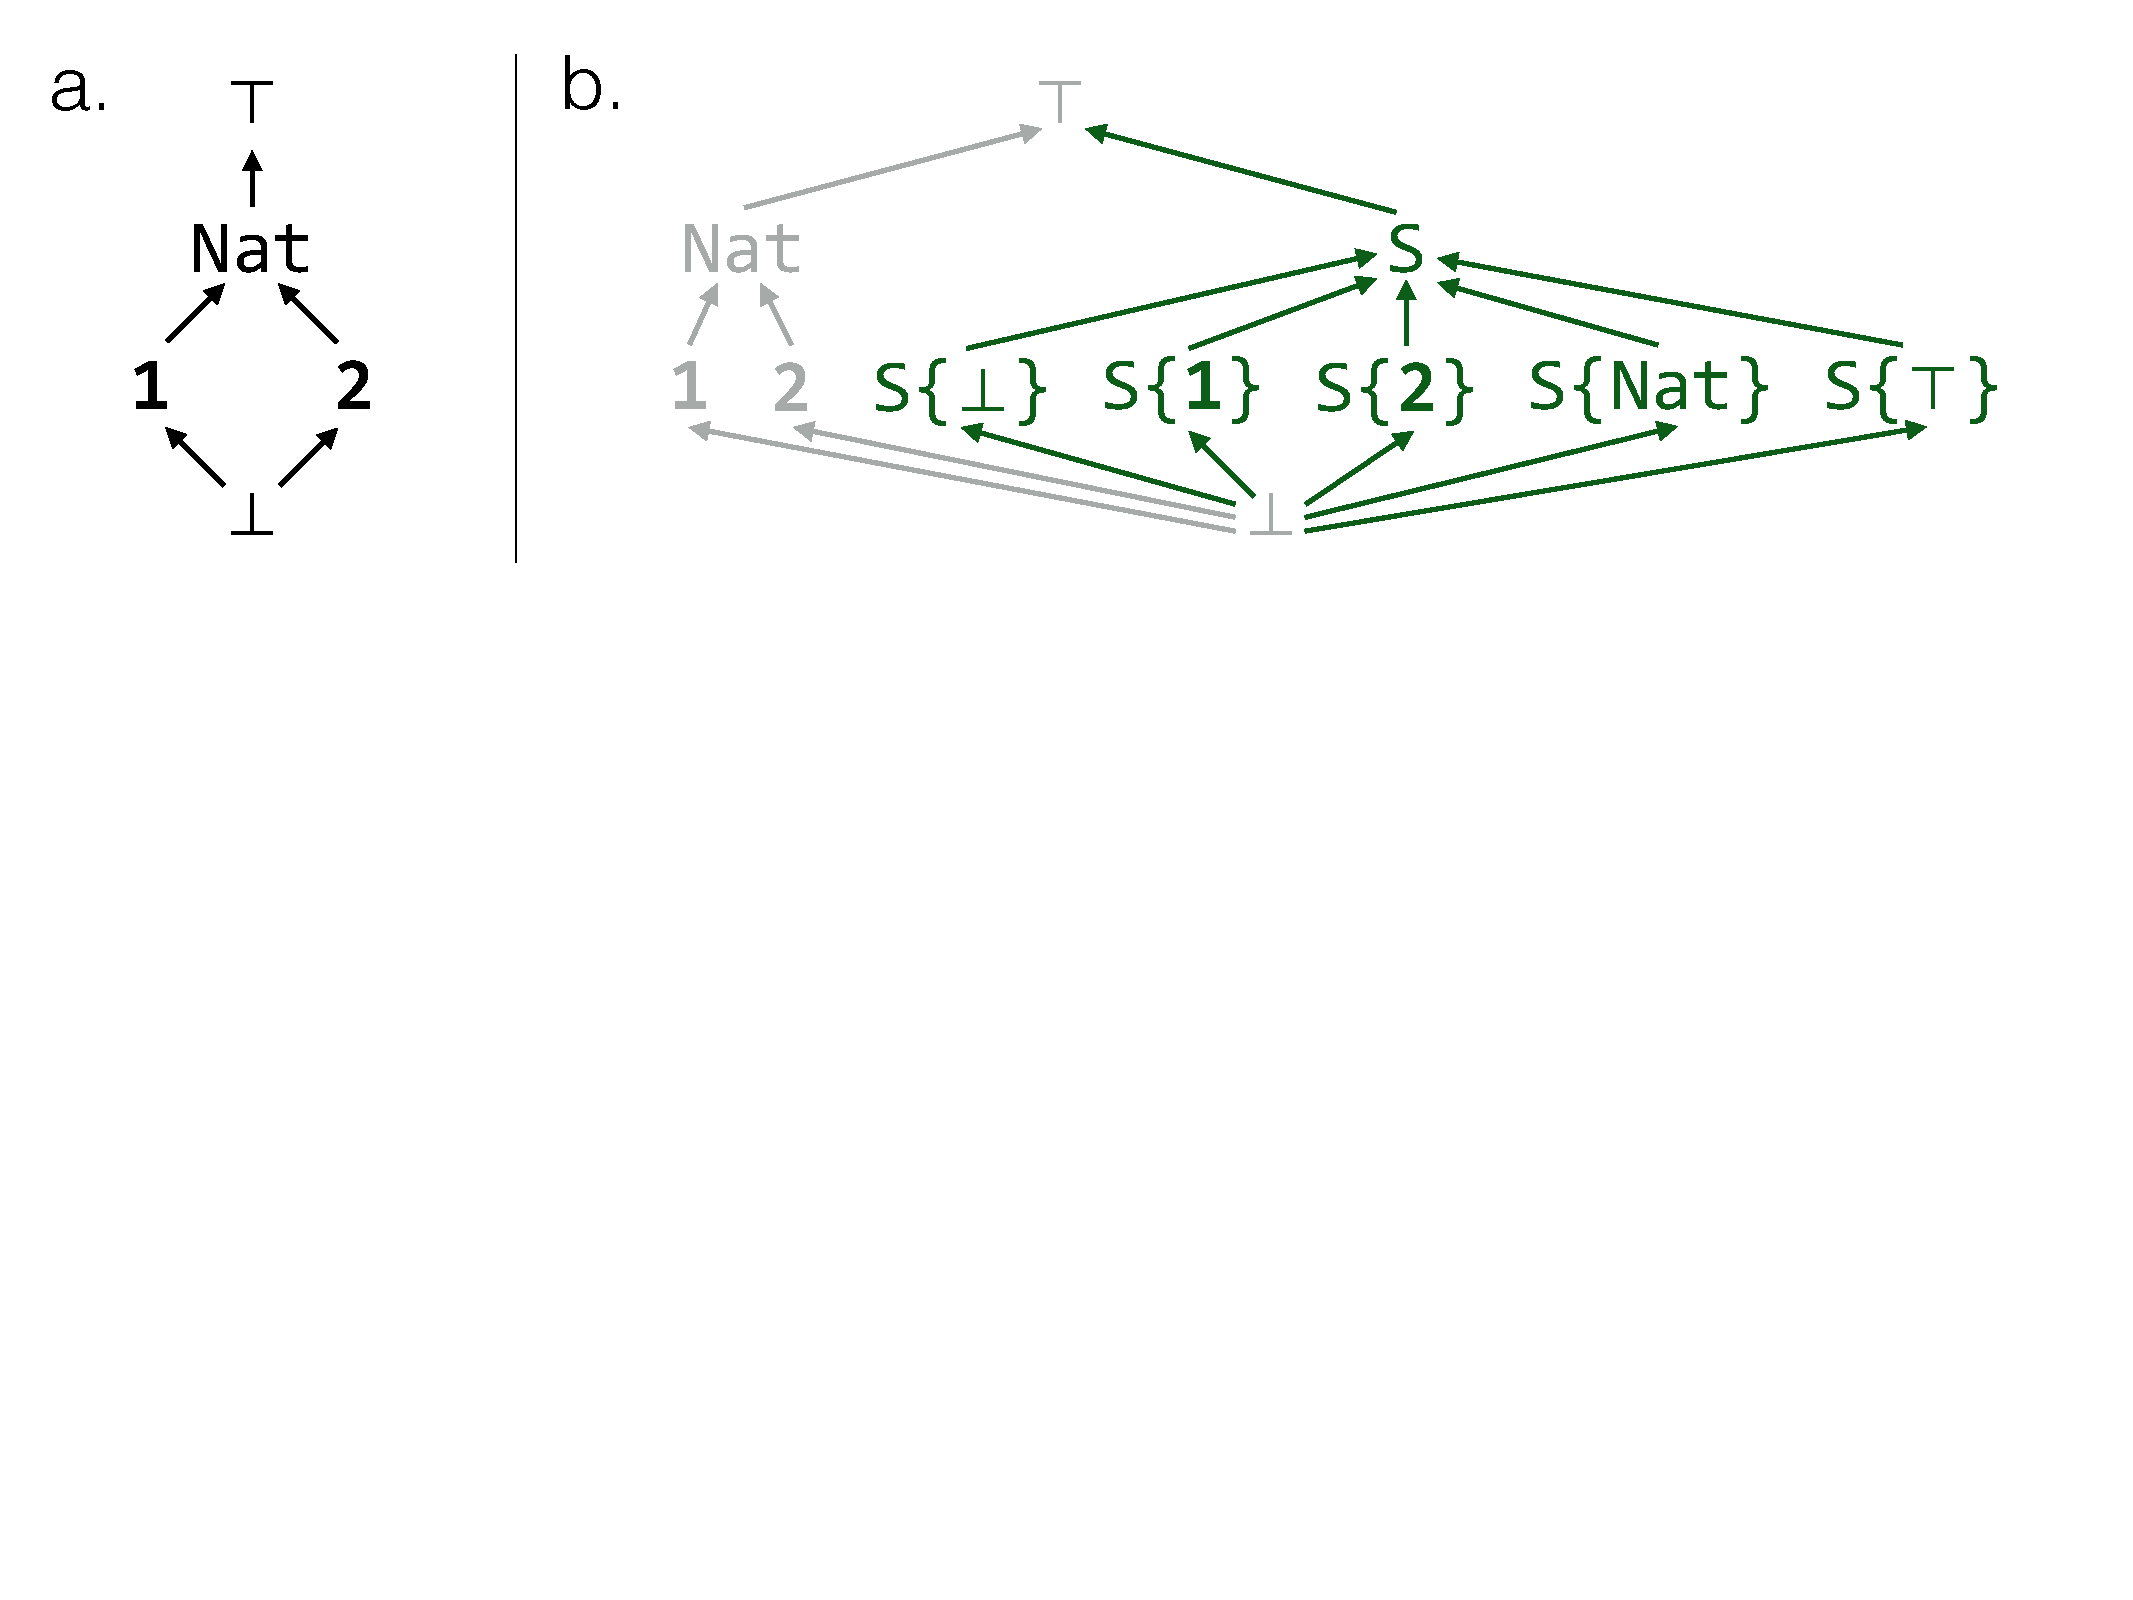
\includegraphics[width=\columnwidth]{fig-lattice}
	\caption{
		\textbf{a.} A simple lattice with bottom type $\bot$, top type
		$\top$, singleton types \textbf{1} and \textbf{2}, and their
		supertype \texttt{Nat}.
		\textbf{b.} The same lattice extended with a parametric type
		\texttt{S\{T\}} with no restriction on the type parameter
		\texttt{T}, showing that for each \texttt{T}, invariance
		requires that the corresponding type \texttt{S\{T\}} be a leaf
		type (i.e.\instantiable), even if \texttt{T} itself is not a
		leaf type.}
	\label{fig:lattice}
\end{figure}

%% Second, the example of Figure~\ref{fig:lattice} illustrates how invariance of
%% type parameters requires parametric types to be instantiable with any type
%% parameter, regardless of whether the parameter corresponds to an abstract or
%% concrete type. The rationale for this behavior allows for the Julia compiler to
%% reason about different representations, and is perhaps best explained in the
%% context of arrays. For arrays, the type parameter describes the set of possible
%% element types~\cite{Bezanson2014}. An \verb|Array{Float64}|
%% can only contain concrete elements of type \verb|Float64|, whereas an
%% \verb|Array{Real}| can contain elements that are subtypes of \verb|Real| such
%% as \verb|Int|, \verb|Float64| or even \verb|Rational|. The former array
%% consists of concrete immutable elements and can be reified with a single
%% pointer to a contiguous memory block. This representation allows the tags for each element to be elided,
%% resulting in a memory layout which can interoperate with C or Fortran code.
%% The latter array can store more diverse objects,
%% but the element type provides no information about the mutability of each
%% element. Consequently, the array must be represented in memory with pointers to
%% boxed elements, so that checks from generated LLVM code can be inserted that
%% call back into the Julia runtime to determine the actual type of the stored
%% element at run-time. Thus describing arrays as parametric types allows
%% different data structures to be used under the hood without any semantic
%% changes imposed on users, thus allowing for more performance in one case and
%% greater flexibility in the other.


%%Subtyping and type parameters combine to provide powerful expressions of
%%polymorphism, similar to those formalized by $\lambda$-calculi such as
%%System~F$_\le$~\cite{Cardelli1985}. However, the interaction of these two
%%Julia languages features can be subtle and confusing. For example, \verb|Real|
%%is not a subtype of \verb|Complex| because for each type \verb|T| that is a
%%subtype of \verb|Real|, there is a corresponding instantiable type
%%\verb|Complex{T}|. None of these correspond to \verb|Real| since there is no
%%\verb|T| such that \verb|Complex{T}| is a one-component number, and each
%%concrete type only has $\bot$ as its subtype.

%%Another more subtle situation arises from parametric invariance: each value of
%%\verb|Complex{Int64}| is a Gaussian integer, i.e., a complex number where each
%%component is an integer, and so each \verb|Complex{Int64}| is in 1:1
%%correspondence with a value in \verb|Complex{Integer}| and also in
%%\verb|Complex{Real}|. Nevertheless, \verb|Complex{Int64}| is a subtype of
%%neither \verb|Complex{Integer}| nor \verb|Complex{Real}| due to parametric
%%invariance. However, all of these are subtypes of \verb|Complex|.

%% The instantiability of parametric types with non-leaf type parameters can lead
%% to subtle performance bottlenecks and reasoning pitfalls. Consider the three
%% \code{Complex} numbers

%% \begin{lstlisting}
%% z1 = Complex{Float64}(0.0, 1.0)
%% z2 = Complex{FloatingPoint}(0.0, 1.0)
%% z3 = Complex{Union(Rational, Integer, Float64)}(0, 1.0)
%% \end{lstlisting}
%% %
%% which are all numerically equivalent (i.e.\ \verb|z1 == z2 == z3|), but not
%% identical in the \textit{egal} sense~\cite{Baker1993} (\verb|===| in Julia).
%% If we inspect the variables using Julia's \verb|dump| command, we get:

%% \begin{lstlisting}
%% julia> dump(z1)
%% Complex{Float64}
%%   re: Float64 0.0
%%   im: Float64 1.0

%% julia> dump(z2)
%% Complex{FloatingPoint}
%%   re: Float64 0.0
%%   im: Float64 1.0

%% julia> dump(z3)
%% Complex{Union(Integer,Float64,Rational{T<:Integer})}
%%   re: Int64 0
%%   im: Float64 1.0
%% \end{lstlisting}
%% %
%% We see that the \verb|::T| tag annotation on a field does not guarantee that
%% the type of a value placed in the field in any given instance of that type is
%% exactly of type \verb|T|, merely that it is a subtype of \verb|T|. Only for
%% \verb|z1| can the compiler elide the run-time type checks and hence represent
%% \verb|z1| with the fields contiguous in memory without indirection, which
%% increases the performance of code working on \verb|z1| relative to \verb|z2|
%% and \verb|z3|. Nevertheless, all three are fully-fledged \verb|Complex|
%% numbers and support all the semantics associated with the \verb|Complex| type.
%% In this way, Julia allows for a meaningful compromise being flexibility and
%% performance.

\subsection{Function types}

Julia is higher-order; functions can be passed to and returned from other functions.
However, the language currently does not have function (arrow) types.
The reason for this is that a Julia function need not have a useful canonical return type.
We could consider every function to have return type \verb|Any|, but this is not terribly revealing.
Return types based on Julia's type inference would not be predictable, as inference is heuristic and best-effort.
Future compiler improvements can make inferred types more specific, and this should not effect program behavior (only performance).

Julia does support \emph{nominal} function types --- a data type may implement
the \verb|call| generic function, allowing it to be used anywhere a function
can be used.

\subsection{Type conversion}

While Julia code can be written without
explicitly reasoning about types, the ability to do so is sometimes necessary for
understanding code performance issues. Julia provides the \verb|convert(T, x)|
function which converts a value \verb|x| to its corresponding representation in
the type \verb|T|. This is a generic function like any other, but since
\verb|T| is typically a compile-time constant, \verb|convert| this can serve
as a mechanism for limiting polymorphism in code where performance
considerations are important.

The idea of converting a value of type \verb|A| to type \verb|B|
does not naturally belong to one type or the other, which favors multiple
dispatch over classes. Conversion also benefits from open extension:
mathematical objects often have embeddings in multiple domains, not all of
which might be known or desired by the original author of some code. For
example, numbers can be embedded in matrices with diagonal matrices, but not
all users are likely to find this correspondence helpful.


\section{Generic functions and multimethods}

Mathematical thought is
naturally polymorphic. Multimethods are a natural mechanism for capturing such
polymorphism~\cite{Bezanson2014b,Chen2014}. Consider an operation as
fundamental as multiplication: an expression like \verb|a*b| can mean:

\begin{itemize}
	\item a matrix-matrix product,
	\item a matrix-vector product, or
	\item a scalar-vector product,
\end{itemize}
%
to name just a few possibilities. A generic function system supporting
multimethods allows for the \verb|*| function to be polymorphic, expressing a
common metaphor for different kinds of multiplication which can be
disambiguated by the types of \verb|a| and \verb|b|. In contrast, languages
supporting only classes cannot capture the full extent of polymorphism in
\verb|*| in method dispatch: as classes inherently support only single dispatch
on the first argument, each method \verb|*| defined for each class \verb|a|
must contain different code blocks for each possible type of \verb|b|, thus in
practice requiring multiple dispatch to be emulated using virtual methods and
visitor patterns~\cite{designpatterns}. Furthermore, implementing binary methods can
require knowing the internal representation of both objects \verb|a| and
\verb|b|, especially for performance reasons~\cite{Bruce1995}. Such knowledge
fundamentally corrupts the abstraction of class-based encapsulation, as the
methods associated with \verb|a| must know implementation details of all
possible objects \verb|b| that \verb|a| may interact with.
In contrast, there is no abstraction leak associated with allowing a generic
function \verb|*| knowledge about the internal representations of the types it
works on.

Multiplication represented by \verb|*| can be extended, for
example, to multiplication between quaternions, or even to $N$-ary
matrix-matrix products, where associativity\footnote{Neglecting the lack of
exact associativity in some fields such as floating-point numbers.} allows
matrix-matrix products to be regrouped so as to minimize the total memory
footprint and operation count~\cite{Hu1984}.

The extensibility of Julia's generic functions and types allow users to
define new behaviors that intermix new types and new functions. The price we pay
for such flexibility, of course, is that dynamic function dispatch incurs
greater overhead: unlike in a single dispatch language, multiple lookups in
method tables may be necessary to determine which method is most
appropriate~\cite{Bruce1995}. Type inference is
useful for minimizing or even eliminating the
overhead associated with multiple dispatch.

Many of the use cases for multiple dispatch could potentially be addressed
by operator overloading as in C++. However C++ forces programmers to choose
which operations will use dynamic dispatch (via virtual methods), which will
use templates, and which will use function overloading. We conjecture that
this choice can be an unwelcome productivity drain. For example, the
syntactic difference between function calls and method calls could require
code to be rewritten when requirements change, or could lead to APIs that
are not consistent about when method calls are used.


%Another, subtler point is that unlike other object models, generic functions
%provide no encapsulation guarantees, since they are allowed to peer into the
%internal representation of types. Consequently, type safety requires stringent
%criteria on the allowed variances of types~\cite{Allen2011}.


%% NOTE: This section is actually very good but I don't think we can use it unless
%% we show what this feature is good for. Jiahao has said he doesn't feel this is
%% all that useful for technical computing, so better to leave it out.

%% \subsection{Diagonal dispatch}

%% Diagonal dispatch is a special refinement of method dispatch that occurs when a
%% type parameter appears in more than position in the method signature, e.g.:

%% \begin{lstlisting}
%% f{T}(x::T, y::T)
%% \end{lstlisting}
%% %
%% Diagonal dispatch occurs only for concrete types \verb|T|. For example,
%% \verb|f(1, 2)| works as the arguments are of type \verb|(Int, Int)|, but not
%% \verb|f(1, 2.0)| as the arguments are of type \verb|(Int, Float64)|, even
%% though that tuple type is a subtype of \verb|(T, T)| where
%% \verb|T = Union(Int,| \verb|Float64)| or any larger common supertype of \verb|Int| and
%% \verb|Float64|. Thus for diagonal dispatch to match only concrete \verb|T|s,
%% the tuple of arguments is treated \textit{not} covariantly, but rather,
%% \textit{invariantly}. Although this is an unusual special-casing of tuple
%% behavior, the greater specificity allowed by invariance makes diagonal dispatch
%% more useful in practice by matching only concrete types, particularly when
%% \verb|T| appears multiple times in the method signature, e.g.\
%% \verb|f{T}(x::T, y::T, z::T)| or even \verb|f{T}(xs::T...)|.

%% The \textit{diagonal} nature of diagonal dispatch is apparent when considering
%% the dispatch table for the method \verb|f{T}| \verb|(x::T, y::T)|: when written
%% out as a table with all possible types of \texttt{x} and \texttt{y} along the
%% rows and columns as shown in Table~\ref{tab:diagonal}, the method dispatches
%% only along the diagonal of the table.

%% \begin{table}
%% \begin{tabular}{c | c c c c c}
%% 	& \verb|Int| & \verb|Float64| & \verb|Bool| & \verb|Real| & $\cdots$ \\ \hline
%% 	\verb|Int|     & \checkmark &  &  &  & \\
%% 	\verb|Float64| &  & \checkmark &  &  & \\
%% 	\verb|Bool|    &  &  & \checkmark &  & \\
%% 	\verb|Real|    &  &  &  &  & \\
%% 	$\vdots$       &  &  &  &  &
%% \end{tabular}
%% \caption{Dispatch table for the function \texttt{f} with method
%% \texttt{f\{T\}(x::T, y::T)}, showing that dispatch occurs only along the
%% diagonal with all possible types of \texttt{x} and \texttt{y} along the rows
%% and columns.}
%% \label{tab:diagonal}
%% \end{table}


\section{Type inference}
\label{sec:inference}

It is well known that type inference can be used to move tag manipulations
and method lookup to compile time, thus eliminating most overhead from
the execution of dynamically-typed code~\cite{Kaplan1977,Kaplan1980}.
Data flow type inference~\cite{Nielson2005,Khedker2009}
is especially useful in this context, as its
flow-sensitivity yields good type information even if the type of a program
variable is different at different points in the code.
Data flow analysis, particularly in the
forward direction, captures the human intuition of how programs work:
values start at the top and move through the program step by step.
Another advantage of this approach is that it is \emph{not} speculative:
it yields correct deductions about types that, in the best case, allow
overhead to be removed entirely. This property is important to technical
users, who need languages that can match the performance of C and Fortran.

Unfortunately, data flow type inference can be defeated
by dynamic language programs that are too ``type complex''. If the library
functions used might return too many different types, or there are too
many paths through user code, the resulting type information might not
be useful.

Julia was designed to help mitigate this problem. By encouraging
code to be written in small pieces labeled with type information (for
dispatch), it is easier for the compiler to rule out execution paths
that do not actually occur.

Type inference in Julia occurs after code is parsed, macro-expanded, and
lowered into a static single assignment (SSA) intermediate representation
(IR)~\cite{Alpern1988,Rosen1988} that facilitates data flow
analysis~\cite{Cousot1977,Cousot2000,Nielson2005} and is relatively
straightforward to map onto LLVM IR~\cite{Lattner2004}. Julia uses Mohnen's algorithm
for abstract interpretation~\cite{Cousot1992} which works directly on the SSA
IR~\cite{Mohnen2002}. The abstract semantics are described internally using
transfer functions (a.k.a.\ t-functions or flow functions), which approximate
program semantics by inferring possible output types based on the types of
the inputs.

In practice, the expressiveness of Julia's late binding semantics, combined
with the presence of potentially infinite types such as varargs tuples
\verb|(T...)|, complicate type inference.
%The combination of late binding and
%the ability to use generic functions as type parameters also means that the
%general type inference problem is undecidable, as was proved for the System F
%calculus~\cite{Wells1999}.
Therefore practical type inference necessitates
widening heuristics, which reduce computational costs and guarantee termination
in the presence of recursive types~\cite{Cousot1992a}. Examples of such
heuristics include widening (pessimizing) type unions and tuple types which
exceed a certain length, and limiting the maximal depths of types
and tuples analyzed.
%Widening operations are not guaranteed to be monotonic,
%i.e.\ the ordering of approximations may no longer be preserved, and hence the
%fixed point computed by abstract interpretation is not guaranteed to be
%minimal even in a formally monotonic data flow framework~\cite{Cousot1992}.
%Thus the inferred types are not necessarily the least upper bounds on the
%possible values~\cite{Kaplan1977,Kaplan1980}.

Julia provides language features to help users inspect the results of type
inference and specify additional type information where necessary to sharpen
the types of variables.

\begin{enumerate}

	\item The base library provides introspection functions like
	\verb|code_typed|, which allow users to inspect generated type
	annotations and avoid second-guessing the compiler's intentions.

	\item Variables can also be given explicit \textbf{type annotations};
	changing \verb|x = 0| to \verb|x::Float64 = 0| declares \verb|x| to be
	of type \verb|Float64| within the current scope, and all assignments
	\verb|x = _| implicitly call the type conversion function
	\verb|convert(Float64, _)|.

	\item Expressions can be given \textbf{type assertions}; changing
	\verb|x += y| to \verb|x += y :: Int| asserts that \verb|y| must be of
	type \verb|Int| or otherwise raise a run-time error.

\end{enumerate}
%
External packages like \package{TypeCheck.jl} and \package{Lint.jl} provide
further static analyses which are useful for detecting type-related issues.


\section{Applications in technical computing}

In this section, we describe how the type system, generic functions and type
inference interact in Julia code for scientific computations in base library
code as well as registered packages.

\subsection{Type promotion}

The type system and generic function system allow for type promotion rules to
be specified in the base library rather than be hard-coded into a given
implementation~\cite{Bezanson2012a}. For example, simple arithmetic functions
on general numeric types in Julia's base library contain methods of the form:

\begin{lstlisting}
+(x::Number, y::Number) = +(promote(x,y)...)
*(x::Number, y::Number) = *(promote(x,y)...)
-(x::Number, y::Number) = -(promote(x,y)...)
/(x::Number, y::Number) = /(promote(x,y)...)
^(x::Number, y::Number) = ^(promote(x,y)...)
\end{lstlisting}

For example, an operation like \verb|2 * 3.4| is evaluated under the hood as
follows:

\begin{lstlisting}
*(2, 3.4) = *(promote(2, 3.4)...)
          = *(convert(promote_type(Int,Float64),2),
	      convert(promote_type(Int,Float64),3.4))
          = *(convert(Float64,2), convert(Float64,3.4))
	  = *(2.0, 3.4)
	  = 6.8
\end{lstlisting}
%
where \verb|promote(x, y)| promotes the values \verb|x| and \verb|y| to
numerically equivalent values of a common supertype, and
\verb|promote_type(S,T)| computes a common supertype of \verb|S| and \verb|T|.
The latter calls a custom promotion rule, if defined, and defaults otherwise to
the join \verb|S|$\vee$\verb|T|.

Type promotion allows for different functions and methods to share a common and
consistent logic for polymorphism. The implementation of type promotion
leverages the type system to allow for greater code reuse across different
methods and functions. Furthermore, it is a part of the Julia language which
can be built entirely from other language constructs.


\subsection{Numerical linear algebra library}

Designing a general-purpose linear algebra library involves several different
layers of complexity, and has been described as implementing the following
meta-program~\cite{Demmel2007}:

{\small
\begin{verbatim}
(1) for all linear algebra problems
    (linear systems, eigenproblems, ...)
(2)  for all matrix types
     (general, symmetric, banded, ...)
(3)   for all data types (real, complex,
      single, double, higher precision)
(4)    for all machine architectures and
       communication topologies
(5)     for all programming interfaces
(6)      provide the best algorithm(s) available
         in terms of performance and accuracy
         (``algorithms'' is plural because
         sometimes no single one is always best)
\end{verbatim}
}
%
The six-tiered hierarchy neatly delineates how the basic collection of linear
algebra problems (1) have to be specialized by data representation (2--3) and
machine details (4), which are then used to decide which specific algorithms
(5--6) to use.

Many systems provide optimized implementations of standard libraries for
numerical linear algebra like BLAS (Basic Linear Algebra Subprograms) and
LAPACK (Linear Algebra PACKage)~\cite{lapack}. Computational routines can be
customized for individual microarchitectures and can reach a large fraction of
theoretical peak FLOPS. However, these libraries inherit archaic Fortran 77
interfaces and hence tend to restrict routine names to six letters or shorter.
When combined with the lack of polymorphism in Fortran, the names are terse and
cryptic to nonexperts: a typical routine like \verb|DSTEV| solves the
eigenvalue problem (\verb|EV|) for symmetric tridiagonal matrices (\verb|ST|)
with double precision floating point entries (\verb|D|), and furthermore takes
eight positional arguments specifying the inputs, outputs, computation mode,
and scratch variables. The lack of polymorphism results in redundancy due to
lack of code reuse, which hinders the implementation of new algorithms (which
have to be reimplemented for each level of floating-point precision) and new
routines for such as mixed-precision and quad precision routines (which must
implement all the existing algorithms).

The code redundancy problem is largely ameliorated with the combination of type
polymorphism and dynamic multiple dispatch. The six-tiered hierarchy above maps
naturally onto different language constructs in Julia as follows:

\vspace{12pt}
\begin{tabular}{c l l}
	\hline
	Tier & Description & Language construct \\ \hline
	1 & linear algebra problems & generic function \\
	2 & matrix types & parametric types \\
	3 & data types & type parameter \\
	4 & machine architectures & method body \\
	5 & programming interfaces & generic function \\
	6 & (poly)algorithms & method body \\ \hline
\end{tabular}
\vspace{12pt}

The generic function system allows for fast specializations and generic
fall-backs to coexist, thus allowing for speed when possible and flexibility
otherwise. For example, Julia provides generic fall-back routines to do matrix
computations over arbitrary fields of element types, providing the ability to
compute on numeric types which are not mappable to hardware floating point
types. This can be useful to perform matrix computations in exact rational
arithmetic or software-emulated higher precision floating point arithmetic to
verify the implementations of algorithms or to detect the possibility of
numerical instability associated with roundoff errors. These general purpose
routines coexist with BLAS and LAPACK wrappers, thus allowing dispatch onto
performant code when available, and general code otherwise. User code can be
written that will work regardless of element type (Tier 3), and can be tuned
for performance later.

\subsection{Generic linear algebra}

Code for technical computing often sacrifices abstraction for performance,
and is less expressive as a result. In contrast, mathematical ideas are
inherently polymorphic and amenable to abstraction. Consider a simple example
like multiplication, represented in Julia by the \lstinline|*| operator.
\lstinline|*| is a generic function in Julia, and has specialized methods for
many different multiplications, such as scalar--scalar products, scalar--vector
products, and matrix--vector products. Expressing all these operations using
the same generic function captures the common metaphor of multiplication.

\subsection{Bilinear forms}

Julia allows user code to extend the \lstinline|*| operator, which can be
useful for more specialized products. One such example is bilinear forms, which
are vector--matrix--vector products of the form
%
\begin{equation}
\gamma = v^\prime M w = \sum_{ij} v_i M_{ij} w_j
\end{equation}
%
This bilinear form can be expressed in Julia code as
%
\begin{lstlisting}
function (*){T}(v::AbstractVector{T},
                M::AbstractMatrix{T},
                w::AbstractVector{T})
    if !(size(M,1) == length(v) &&
         size(M,2) == length(w))
        throw(BoundsError())
    end
    $\gamma$ = zero(T)
    for i = 1:size(M,1), j = 1:size(M,2)
        $\gamma$ += v[i] * M[i,j] * w[j]
    end
    return $\gamma$
end
\end{lstlisting}
%
The newly defined method can be called in an expression like
\lstinline|v * M * w|, which is parsed and desugared into an ordinary function
call \lstinline|*(v, M, w)|. This method takes advantage of the result being a
scalar to avoid allocating intermediate vector quantities, which would be
necessary if the products were evaluated pairwise like in $v^\prime(Mw)$ and
$(v^\prime M) w$. Avoiding memory allocation reduces the number of
heap-allocated objects and produces less garbage, both of which are important
for performance considerations.

The method signature above demonstrates two kinds of polymorphism in Julia.
First, both \lstinline|AbstractVector| and \lstinline|AbstractMatrix| are
abstract types, which are declared supertypes of concrete types. Examples of
subtypes of \lstinline|AbstractMatrix| include \lstinline|Matrix| (dense
two-dimensional arrays) and \lstinline|SparseMatrixCSC| (sparse matrices stored
in so-called compressed sparse column format). Thus the method above is defined
equally for arrays of the appropriate ranks, be they dense, sparse, or even
distributed.  Second, \lstinline|T| defines a type parameter that is common to
\lstinline|v|, \lstinline|M| and \lstinline|w|. In this instance, \lstinline|T|
describes the type of element stored in the \lstinline|AbstractVector| or
\lstinline|AbstractMatrix|, and the \lstinline|{T}(...{T}...{T})| syntax
defines a family of methods where \lstinline|T| is the same for all three
arguments. The type parameter \lstinline|T| can also used in the function body;
here, it is used to initialize a zero value of the appropriate type for
$\gamma$.

The initialization statement \lstinline|$\gamma$ = zero(T)| requests a zero
element of the appropriate type.
In Julia this is important because using a zero value of a different type can
cause a different method to be called.
%allows Julia's compiler
%to generate \textbf{type stable} code.
If \lstinline|T| is any concrete %immutable
type, e.g.\ \lstinline|Float64| (64-bit floating point real numbers), then
Julia's just-in-time compiler can analyze the code statically to remove type
checks.  For example, in the method with signature
\lstinline|*{Float64}(v::AbstractVector{Float64}, M::AbstractMatrix{Float64}, w::AbstractVector{Float64})|,
the indexing operations on $v$, $M$ and $w$ always return \lstinline|Float64|
scalars. Furthermore, forward data flow analysis allows the type of $\gamma$
to be inferred as \lstinline|Float64| also, since floating point numbers are
closed under addition and multiplication. Hence, type checks and method
dispatch for functions like \lstinline|+| and \lstinline|*| within the function
body can be resolved statically and eliminated from run time code, allowing
fast code to be generated.

Were we to replace the initialization with the similar-looking
\lstinline|$\gamma$ = 0|, we would have instead a \textbf{type instability}
when \lstinline|T = Float64|. Because $\gamma$ is initialized to an
\lstinline|Int| (native machine integer) and it is incremented zero or more
times by a \lstinline|Float64| in the \lstinline|for| loop, the type of
the variable can change at run time.
In fact, the result type will depend on the size of the input array $M$,
which is only known at run time.
Julia allows this behavior, and our
compiler infers the type of $\gamma$ to be \lstinline|Union(Int,Float64)|,
which is the least upper bound on the actual type of $\gamma$ at run time.
%However, in such cases it is not generally possible to generate optimal code.
As a result, not all type
checks and method dispatches can be hoisted out of the loop body, resulting
in slower execution.


\subsection{Matrix equivalences}

Matrix equivalences are another example of specialized product that users may
want. Two $n\times n$ matrices $A$ and $B$ are considered equivalent if there
exist invertible matrices $V$ and $W$ such that $B = V * A * W^\prime$.
Oftentimes, equivalence relations are considered between a given matrix $B$ and
another matrix $A$ with special structure, and the transformation
$(W^\prime)^{-1} \cdot V^{-1}$ can be thought of as changing the bases of the
rows and columns of $B$ to uncover the special structure buried within as $A$.
Matrices with special structure are ubiquitous in numerical linear algebra. One
example is rank-$k$ matrices, which can be written in the outer product form $A
= X Y^\prime$ where $X$ and $Y$ each have $k$ columns. Rank-$k$ matrices may be
reified as dense two-dimensional arrays, but the matrix--matrix--matrix product
$V * A * W^\prime$ would take $O(n^3)$ time to compute. Instead, when $k \ll
n$, the product be computed more efficiently in $O(kn^2)$ time, since
%
\begin{equation}
V A W^\prime = V (X Y^\prime) W^\prime = (V X) (W Y)^\prime
\end{equation}
%
and the result is again a rank-$k$ matrix. Furthermore, we can avoid
constructing $W^\prime$, the transpose of $W$, explicitly. Therefore in some
cases, it is sensible to store $A$ as the two matrices $X$ and $Y$ separately,
rather than as a reified 2D array.

Julia allows users to encapsulate $X$ and $Y$ within a specialized type:
%
\begin{lstlisting}
type OuterProduct{T}
	X :: Matrix{T}
	Y :: Matrix{T}
end
\end{lstlisting}
%
Defining the new \lstinline|OuterProduct| type has the advantage of grouping
together objects that belong together, but also enables dispatch based on the
new type itself. We can now write a new method for \lstinline|*|:
%
\begin{lstlisting}
*(V, M::OuterProduct, W) = OuterProduct(V*M.X, W*M.Y)
\end{lstlisting}
%
This method definition uses a convenient one-line syntax for short definitions
instead of the \lstinline|function ... end| block. This method also does not
annotate \lstinline|V| or \lstinline|W| with types, and so they are considered to
be of the top type $\top$ (\lstinline|Any| in Julia). This method may be called
with any $V$ and $W$ which support premultiplication: so long as
\lstinline|V*M.X| and \lstinline|W*M.Y| are defined and produce matrices of the
same type, then the code will run without errors (``duck typing'').
This flexibility is
convenient since $V$ and $W$ can now be scalars or matrixlike objects which
themselves have special structures, or even more generally could represent
linear maps that are not stored explicitly, but rather defined implicitly
through their actions when multiplying a \lstinline|Matrix| on the left.

The preceding method shows that Julia does not require all method arguments to
have explicit type annotations. Instead, dynamic multiple dispatch allows the
argument types to be determined from the arguments at run time.
Julia's just-in-time compiler will be invoked when the method is first
called, so that static analyses can be performed.
%Dynamic dispatch thus gives us the ability to write highly generic code while
%still allowing method specialization on methods that are actually
%dispatched upon at run time.

We can now proceed to define a new type and method

\begin{lstlisting}
type RowPermutation
	p::Vector{Int}
end

*($\Pi$::RowPermutation, M::Matrix) = M[$\Pi$.p, :]
\end{lstlisting}
%
whose action can be thought of as multiplying by a permutation matrix on the
left, resulting in a version of $M$ with the rows permuted. Now, the following
user code
%
\begin{lstlisting}
n = 10
k = 2
X = randn(n, k) #Random matrix of Float64s
M = OuterProduct(X, X)
p = randperm(n) #Random permutation of length n
$\Pi$ = RowPermutation(p)
M2 = $\Pi$ * M * $\Pi$
\end{lstlisting}
%
will dispatch on the appropriate methods of \lstinline|*| to produce the same
result \lstinline|M2| as
\begin{lstlisting}
M2 = OuterProduct(M.X[p, :], M.Y[p, :])
\end{lstlisting}
%
In other words, the specialized method
\lstinline|*(::RowPermutation, ::OuterProduct{Float64}, ::RowPermutation)|
is compiled only when it is first invoked in the creation of
\lstinline|M2|, since it follows from composing the method defined with
signature \lstinline|*(::Any, ::OuterProduct, ::Any)| with the argument tuple
of type \lstinline|(RowPermutation, OuterProduct{Float64}, RowPermutation)|.

\subsection{Matrix factorization types}

Julia's base linear algebra library also provides extensive support for matrix
factorizations, which are indispensable for reasoning about the
interdependencies between matrices with special properties and the numerical
algorithms that they enable~\cite{Golub2013}. Many algorithms for numerical
linear algebra involve interconversions between general matrices and similar
matrices with special matrix symmetries. For many purposes, it is convenient to
reason about the resulting special matrix, together with the matrix performing
the transformation, as a single mathematical object rather than two separate
matrices. Such an object represents a matrix factorization, and is essentially
a different data structure that can represent the same content as a matrix
represented as an ordinary two-dimensional array.

The exact matrix factorization object relevant for a given linear algebra
problem depends on the symmetries of the starting matrix and also the
underlying field of matrix elements (i.e.\ whether the matrix contains real
numbers, complex numbers, or something else). In some use cases, these
properties may be known by the user as part of the problem specification, and
in other cases they may be unknown. Some properties, like whether a
matrix is triangular, can be deduced by inspecting the matrix elements for
$O(N^2)$ cost. Others, like whether a matrix is positive definite, require an
$O(N^3)$ computation in the general case, and is most efficiently determined by
attempting to compute the Cholesky factorization.

The resulting algorithm for determining a useful matrix factorization has to
capture the interplay between allowing the user to specify additional matrix
properties and attempting to automatically detect useful properties when the
additional cost of doing so is not prohibitive. The general case is implemented
in Julia's base library by the \verb|factorize| function, and typifies the
complexity associated with numerical codes:

\begin{lstlisting}
function factorize{T}(A::Matrix{T})
	m, n = size(A)
	if m != n
		# A is rectangular
		# Can the result of a QR factorization be represented
		# using a floating point type supported by BLAS?
		BlasFloat = Union(Float32,Float64,Complex64,Complex128)
		rt = zero(T) / sqrt(zero(T) + zero(T))
		can_use_BlasFloat = isa(rt, BlasFloat)
		# Factorize into pivoted QR form where possible,
		# otherwise compute (unpivoted) QR form
		return qrfact(A, pivot=can_use_BlasFloat)
	end
	# A is square
	# The factorization of a 1x1 matrix is just itself
	m == 1 && return A[1]
	utri = istriu(A)          # upper triangular?
	utri1 = ishessenbergu(A)  # upper Hessenberg?
	sym = issym(A)
	herm = ishermitian(A)
	ltri = istril(A)          # lower triangular?
	ltri1 = ishessenbergl(A)  # lower Hessenberg?
	if ltri && utri
		return Diagonal(A)
	elseif ltri && utri1
		return Bidiagonal(diag(A), diag(A, -1), false)
	elseif ltri
		return Triangular(A, :L)
	elseif ltri1 && utri
		return Bidiagonal(diag(A), diag(A, 1), true)
	elseif ltri1 && utri1
		if (herm && (T <: Complex)) || sym
			M = SymTridiagonal(diag(A), diag(A, -1))
			# _may_ be factorizable into
			# LDL' Cholesky form
			try
				return ldltfact!(M)
			end
		end
		# A is tridiagonal
		M = Tridiagonal(diag(A,-1), diag(A), diag(A,1))
		# Factorize into tridiagonal LU form
		return lufact!(M)
	elseif utri
		return Triangular(A, :U)
	elseif herm
		# _may_ be factorizable into Cholesky form
		try
			return cholfact(A)
		end
		# else use general Hermitian factorization
		return factorize(Hermitian(A))
	elseif sym
		# use general Symmetric factorization
		return factorize(Symmetric(A))
	else
		# A is square but has no other symmetries
		# Factorize into LU form
		return lufact(A)
	end
end

# Factorize a Hermitian or Symmetric matrix into
# Bunch-Kaufman form as computed by bkfact
typealias HermOrSym Union(Hermitian,Symmetric)

factorize(A::HermOrSym) =
    bkfact(A.data, symbol(A.uplo), issym(A))
\end{lstlisting}

The \verb|factorize| function contains a few interesting features
designed to capture the highly dynamic nature of this computation:

\begin{enumerate}
\item The beginning checks for the ``easy'' properties, i.e.  those that can be
	computed cheaply at run-time by inspecting the matrix elements. The
	presence of one or more of these properties allow the input matrix
	\verb|A| to be classified into several special cases.

\item For many of these special cases (like \verb|Diagonal|), \verb|A| is
	explicitly converted to a special matrix type which allows dispatch on
	efficient specializations of linear algebraic operations that users may
	choose to perform later, such as matrix multiplication.

\item For other special cases (like \verb|Tridiagonal|), it is useful to
	attempt a run-time check for the ``hard'' properties, like positive
	definiteness, which require nontrivial computation. Computing the
	Cholesky factorization serves both as an efficient run-time check to
	detect positive definiteness, whose failure indicates lack thereof, and
	whose success yields a useful \verb|Cholesky| matrix factorization
	object which is useful for further computations such as solving linear
	equations or computing singular value decompositions (SVDs).

\item The \verb|Symmetric| and \verb|Hermitian| cases use control flow
	enabled by dynamic multimethods, as it is common for users to know
	whether the matrices they are working with have these properties.
	Using multimethods allows users to elide all the run-time checks
	in the generic method, skipping directly to the appropriate specialized
	method.

\item The base case contains a nontrivial runtime check to determine if the
	element type of \verb|A{T}| can be represented as a
	hardware-representable real or complex floating point number. The
	\verb|canuseBlasFloat| variable computes the type resulting from
	computations of the form $x / \sqrt{x + x}$, and checks that it is a
	subtype of \verb|BlasFloat|. The reason for this check is that there
	are two variants of the QR factorization: one pivoted, the other not.
	The former is generally preferred for numerical stability but is also
	more difficult to compute, and hence is not yet
	implemented for all possible element types.

\end{enumerate}

In theory, it is possible to combine these structured matrix types under a
tagged union, e.g.\ in an ML-family language. However this would be
less convenient. The problem is that in most contexts,
users are happy to have these objects separated by the type system, but
certain functions like \code{factorize} wish to combine them. It should be
possible to pass the result of such a function directly to an existing
routine that expects a particular matrix structure, without needing to
interpose case analysis to handle a tagged union.

It is also instructive to look more carefully at the methods for \verb|bkfact|,
which is but one of the several factorizations computed in \verb|factorize|:

\begin{lstlisting}
# Compute Bunch-Kaufman factorization,

bkfact{T<:BlasFloat}(A::StridedMatrix{T},
                     uplo::Symbol=:U,
                     sym::Bool=issym(A)) =
    bkfact!(copy(A),uplo,sym)

function bkfact{T}(A::StridedMatrix{T},
                   uplo::Symbol=:U,
                   sym::Bool=issym(A))
    Typ = promote_type(Float32,
                       typeof(sqrt(one(T))))
    bkfact!(Matrix{Typ}(A),uplo,symmetric)
end

# Compute Bunch-Kaufman factorization in-place

# For real symmetric matrices,
# if T is Float32 or Float64
# call LAPACK SSYTRF/DSYTRF routine

function bkfact!{T<:BlasReal}(A::StridedMatrix{T},
		              uplo::Symbol=:U,
			      sym::Bool=issym(A))
    if sym
        error("The Bunch-Kaufman decomposition ",
	      "is only valid for symmetric matrices")
    end
    LD, ipiv = LAPACK.sytrf!(char_uplo(uplo),A)
    BunchKaufman(LD,ipiv,char_uplo(uplo),symmetric)
end

# For complex symmetric matrices,
# call LAPACK CSYTRF/ZSYTRF

# If T is Complex64 or Complex128,
# and the matrix is complex Hermitian
# call the CHETRF/ZHETRF routines

function bkfact!{T<:BlasComplex}(A::StridedMatrix{T},
	    			 uplo::Symbol=:U,
				 sym::Bool=issym(A))
    if sym
        LD,ipiv = LAPACK.sytrf!(char_uplo(uplo),A)
    else
        LD,ipiv = LAPACK.hetrf!(char_uplo(uplo),A)
    end
    BunchKaufman(LD,ipiv,char_uplo(uplo),sym)
end
\end{lstlisting}

The Bunch-Kaufman routines are implemented in two functions: \verb|bkfact|,
which allocates new memory for the answer, and \verb|bkfact!|, which mutates
the matrix in place to save memory. Reasoning about memory use is critical in
numerical linear algebra applications as the matrices may be large.
Reusing allocated memory for matrices also avoids unnecessary copies of data to
be made, potentially minimizing memory accesses and reducing the need to
trigger garbage collection. The base library thus provides the latter for users
who need to reason about memory usage, and the former for users who do not.

The syntax \verb|{T<:BlasReal}| in a method definition implicitly wraps the
signature in a \verb|UnionAll| type. As a result, the method matches all
matrices whose elements are of a type supported by BLAS.



\section{Case study: completely pivoted LU}

Linear algebra is ubiquitous in technical computing applications. At the same
time, the implementation of linear algebra libraries is generally considered a
difficult problem best left to the experts. A popular reference book for
numerical methods famously wrote, for example, that ``the solution of
eigensystems... is one of the few subjects covered in this book for which we do
\textit{not} recommend that you avoid canned routines''~\cite[Section 11.0, p.
461]{Press1992}. While much effort has been invested in making
numerical linear algebra libraries
fast~\cite{lapack,Gunnels2001,OpenBLAS,VanZee2013}, one nevertheless will
occasionally need an algorithm that is not implemented in a
standard linear algebra library.

One such nonstandard algorithm is the completely pivoted LU factorization. This
algorithm is not implemented in standard linear algebra libraries in
LAPACK~\cite{lapack}, as the conventional wisdom is the gains in numerical
stability in complete pivoting is not generally worth the extra effort over
other variants such as partial pivoting~\cite{Golub2013}.  Nevertheless, users
may want complete pivoting for comparison with other algorithms for a
particular use case.
%For example, one may be interested in comparing the
%results of an infinite dimensional LU factorization to its finite-dimensional
%approximation, in which case only the completely pivoted LU is defined in both
%cases~\cite{Townsend2014}.

In this section, we compare implementations and performance of this
algorithm in Julia with other high level languages that are commonly used for
technical computing: MATLAB, Octave, Python/NumPy, and R.
%Second, we
%rewrite the na\"ive Julia implementation for better performance, and
%demonstrate the effects of each transformation on execution time. We believe
%that this work flow reflects typical use cases of high level dynamic languages,
%where users first write na\"ive but verifiably correct implementations, then
%rewrite the implementation until sufficient performance can be achieved.



\subsection{Na\"ive textbook implementation}

Algorithm~\ref{alg:lucompletepiv} presents the textbook description of the LU
factorization with complete pivoting~\cite[Algorithm 3.4.3 (Outer Product LU
with Complete Pivoting), p. 132]{Golub2013}, and below it a direct translation
into a na\"ive Julia implementation. This algorithm is presented in MATLAB-like
pseudocode, and contains a mixture of scalar \lstinline|for| loops and
MATLAB-style vectorized indexing operations that describe various subarrays of
the input matrix $A$. Additionally, there is a description for the subproblem
of finding the next pivot at the start of the loop. Furthermore, the pseudocode
uses the $\leftrightarrow$ operation, denoting swaps of various rows and
columns of $A$. To translate the pivot finding subproblem into Julia, we used
the built-in \lstinline|indmax| function to find the linear index of the value
of the subarray \lstinline|A[k:n, k:n]| which has the largest magnitude, then
used the \lstinline|ind2sub| function to convert the linear index to a tuple
index. The $\leftrightarrow$ operator was implemented using vectorized indexing
operations, as is standard practice in high level languages like MATLAB.



\begin{algorithm}

\caption{Top: Textbook pseudocode describing the $LU$ factorization with
complete pivoting~\cite[Algorithm 3.4.3 (Outer Product LU with Complete
Pivoting), p. 132]{Golub2013}. The matrix $A$ is overwritten in-place with the
$LU$ factors, with $rowpiv$ and $colpiv$ containing the row and column pivots
respectively.
Bottom: An implementation of $LU$ factorization with complete pivoting in Julia,
which returns the result as a tuple. The ! at the end of the function name is
convention for a function with side effects (in this case, mutating $A$).
Unicode characters such as Greek letters and the $\ne$ operator are allowed in
Julia code, allowing for close notational correspondence with the textbook
description of the algorithm.}
\label{alg:lucompletepiv}

\begin{algorithmic}
\For {$k = 1:n - 1$}

    Determine $\mu, \lambda$ where $k \le \mu \le n$,  $k \le \lambda \le n$, so

    $\quad\left|A(\mu, \lambda)\right| = \max\{ \left|A(i, j)\right| : i=k:n, j=k:n \}$

    $rowpiv(k) = \mu$

    $A(k, 1:n) \leftrightarrow A(\mu, 1:n)$

    $colpiv(k) = \lambda$

    $A(1:n, k) \leftrightarrow A(1:n, \lambda)$

    \If{$A(k,k) \ne 0$}

        $\rho = k+1:n$

        $A(\rho, k) = A(\rho, k)/A(k, k)$

        $A(\rho, \rho) = A(\rho, \rho) - A(\rho, k) A(k, \rho)$
    \EndIf
\EndFor
\end{algorithmic}

\hrulefill

\begin{lstlisting}
function lucompletepiv!(A)
	n=size(A, 1)
	rowpiv=zeros(Int, n-1)
	colpiv=zeros(Int, n-1)
	for k=1:n-1
		Asub = abs(A[k:n, k:n]) #Search for next pivot
		$\mu$, $\lambda$ = ind2sub(size(Asub), indmax(Asub))
		$\mu$ += k-1; $\lambda$ += k-1
		rowpiv[k] = $\mu$
		A[[k, $\mu$], 1:n] = A[[$\mu$, k], 1:n]
		colpiv[k] = $\lambda$
		A[1:n, [k, $\lambda$]] = A[1:n, [$\lambda$, k]]
		if A[k,k] $\ne$ 0
			$\rho$ = k+1:n
			A[$\rho$, k] = A[$\rho$, k]/A[k, k]
			A[$\rho$, $\rho$] = A[$\rho$, $\rho$] - A[$\rho$, k] * A[k, $\rho$]
		end
	end
	return (A, rowpiv, colpiv)
end
\end{lstlisting}

\end{algorithm}

For comparison purposes, we also wrote na\"ive implementations in other high
level dynamics languages which are popular for technical computing. Here, we
considered MATLAB~\cite{matlab}, Octave~\cite{octave},
Python~\cite{python}/NumPy~\cite{numpy}, and R~\cite{rlang} (whose codes are
available in the Appendix). The codes were executed on a late 2013 MacBook Pro
running OS X
Yosemite 10.10.2, with Julia 0.4-dev+3970, MATLAB R2014b, Octave 3.8.1, Python
3.4.3 with NumPy 1.9.2 from the Anaconda 2.1.0 distribution, and R 3.1.3. Where
possible, we also tried to run variants with and without JIT compilation. In
MATLAB, the JIT compiler is on by default, but can be turned off with the
command \lstinline|feature accel off|. Octave's JIT compiler is experimental
and off by default, but can be enable with a command line switch. R provides a
JIT compiler in the \lstinline|compiler| library package. We do not have
JIT-compiled results for Python, as at this time of writing, neither PyPy
2.5.0~\cite{Bolz2009} nor Numba 0.17.0 was able to compile the code.\footnote{
The specialized fork of NumPy required to run on PyPy 2.5.0 did not build
successfully on neither Python 2.7.9 nor 3.4.3 on OSX. Numba 0.17.0, with the
\lstinline|@jit(nopython=True)| decorator, threw a
\lstinline|NotImplementedError| exception.}
The results are summarized in Figure~\ref{fig:scaling}, which shows the
near-perfect $O(n^3)$ scaling of the algorithm in each implementation, as well
as in Figure~\ref{fig:naivelangs}, which shows the execution times across the
different languages for a $1000 \times 1000$ matrix of \lstinline|Float64|s
with randomly sampled standard Gaussians.

The results show that the na\"ive Julia implementation performs favorably with
the implementations in Matlab and Octave, all of which are significantly faster
than R's implementation. Python's implementation is somewhat faster, owing to
the rank-1 update step (of \lstinline|A[$\rho$, $\rho$]|)
being done in place. Turning on or off the JIT did not significantly change the
execution times for Matlab, Octave and R.

\begin{figure}
	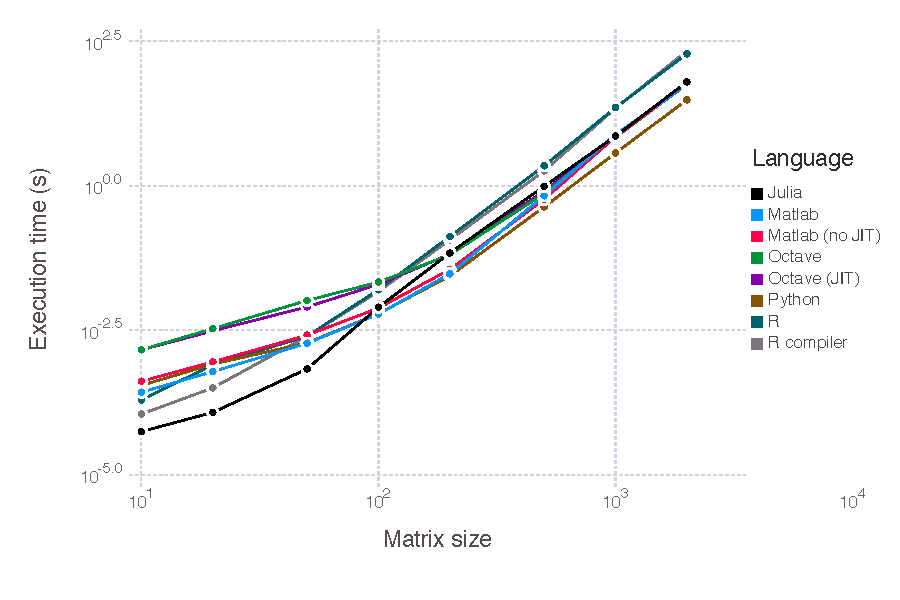
\includegraphics[width=\columnwidth]{data/fig-scaling}
	\caption{Scaling behavior of na\"ive implementations of the completely
	pivoted $LU$ algorithm on $N\times N$ random matrices in Julia, MATLAB,
	Octave, Python/NumPy, and R. By default, MATLAB's JIT compiler is on,
	whereas Octave's and R's are off. Julia code is listed in
	Algorithm~\ref{alg:lucompletepiv}.
	%, and the others are available in the
%Appendix. Plotted with \package{Gadfly.jl}.
}
	\label{fig:scaling}
\end{figure}

\begin{figure}
	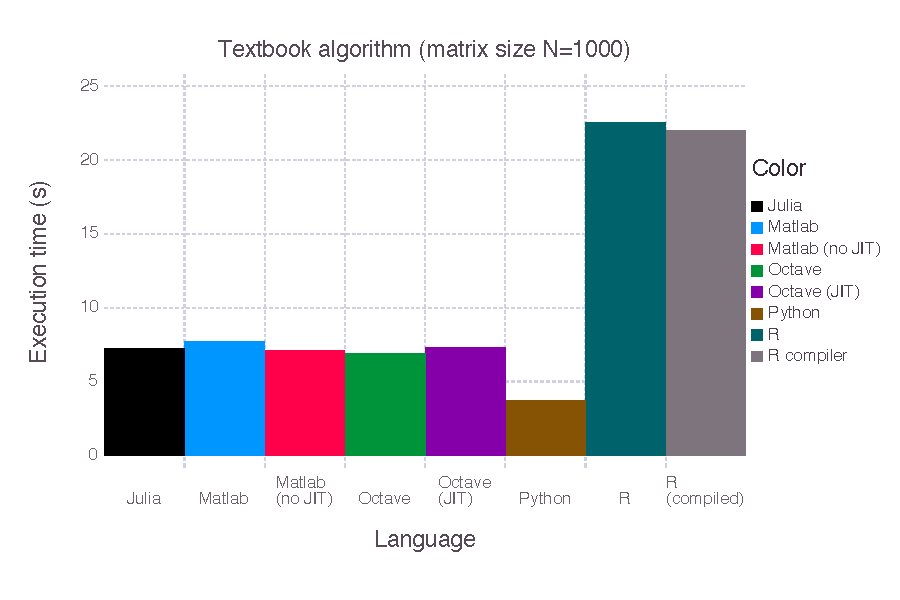
\includegraphics[width=\columnwidth]{data/fig-lang}
	\caption{Execution times of na\"ive implementations of the
	completely pivoted $LU$ algorithm on a $1000\times1000$ random matrix
	in Julia, MATLAB, Octave, Python/NumPy, and R. See Figure~\ref{fig:scaling}
	for further details.}
	\label{fig:naivelangs}
\end{figure}



\subsection{LU decomposition on arbitrary numeric types}

One major advantage to writing the $LU$ factorization code in pure Julia is
that \lstinline|lucompletepiv!| can run on any \lstinline|Matrix{T}|. So long
as the underlying element type \lstinline|T| is closed under the basic
arithmetic operations \lstinline|+|, \lstinline|-|, \lstinline|*|,
\lstinline|/|, \lstinline|abs|, and \lstinline|max|, the algorithm will run
just as it did on \lstinline|Float64| numbers. For example, one could compute
the completely pivoted $LU$ factorization on matrices of fixed point numbers
(provided by the \package{FixedPointNumbers.jl} package), or matrices of
rational numbers (built in \lstinline|Rational| types).

\begin{lstlisting}
using FixedPointNumbers

#Initialize 1000x1000 matrix of 32-bit fixed point 1s with 14 fractional bits
B = ones(Fixed32{14}, 1000, 1000)
lucompletepiv!(B)

#Initialize 1000x1000 matrix of unit rational numbers with 64-bit integer numerators and denominators fixed point 1s with 14 fractional bits
C = ones(Rational{Int64}, 1000, 1000)
lucompletepiv!(C)
\end{lstlisting}

Other interesting examples include the dual and hyperdual numbers provided by
the \package{DualNumbers.jl} and \package{HyperDualNumbers.jl} packages
respectively. Both types of numbers are used for forward mode automatic
differentiation, and can be used with \lstinline|lucompletepiv!| to take
derivatives of the $LU$ factorization itself. Computations over such arbitrary
numeric types would be difficult, if not impossible, in the other languages,
without reimplementing the basic algorithm \lstinline|lucompletepiv!| over and
over again.

While of course it is possible to build in more numeric types to the base
library of any programming language, the approach shown here is more general
by virtue of being extensible by users. Other such numberlike quantities
include colors (in \package{Color.jl}), unitful quantities (in
\package{SIUnits.jl}), interval arithmetic (in \package{ValidatedNumerics.jl}),
finite fields, dates and times (in \lstinline|Base.Dates|), quaternions and
octonions (in \package{Quaternions.jl}, extended precision floating point (in
\package{DoubleDouble.jl}), DNA nucleotides (in \package{BioSeq.jl}), and many
more.



\subsection{Improving the performance of a na\"ive implementation}
One of the reasons why high level languages are slow is that it allows the programmer to express algorithms in terms of array operations. These languages have a limited ability to optimize array expressions and consequently many temporary arrays are allocated during execution of a program.

In languages such as Fortran an C, similar algorithms are usually written without allocating temporary arrays. Some workspace might be required by the algorithm, but memory is then typically allocated once. This makes it possible to compile the code into efficient machine code that is typically much faster than what is possible for higher level array oriented languages.

In Julia, it is possible to express algorithms in terms of array operations, but it is also possible to avoid array allocations and thereby have the compiler optimizing the code to efficient machine code. Hence, a first step in optimizing Julia code is to find the lines during a loop that allocates temporary arrays.

The first line in the loop body makes two unnecessary array copies. The lines that flip columns and rows also allocate temporary arrays which can be avoided and allocations are also made for the scaling and rank one update in the last two lines of the \texttt{if} statement. By writing small auxiliary functions and expanding the scaling and rank one update as loops, it is possible to reduce the number of temporary allocations significantly.

For a square matrix of size 1000, a profiling of the na\"ive implementation reveals that it  allocates more than 12 GB of memory and runs in 4.15 seconds. With the changes mentioned in last paragraph the memory allocation is only 7 MB and the running time reduces to 0.75 seconds. Typically, the avoidance of array allocation amounts to the largest share of speedup when optimizing Julia code, but it is possible to achieve a further speed improvement by annotating the code with two macros that turn off bounds checking on array indexing and allows the compiler to use SIMD registers when possible. This final optimization reduces the running time to 0.4 seconds.

In many cases it is not desired to write out array operations as loops, but it is convenient that this optimization is possible without reimplementing parts of or whole algorithms in C or Fortran first and then compile, link, and call these from the high level language. In Julia, the programmer can optimize incrementally and immediately see eventual speed improvements within a single language.


%%\section{Evaluation}

%%Here we discuss the potential for performance in Julia's design,
%%as well as some shortcomings and challenges we have observed.

%%\subsection{Impact of static analyses on performance}

%%Figure~\ref{fig:timings} shows the relative execution times of benchmark codes
%%representing a wide variety of scientific applications, when various optimizations
%%and analyses are successively turned off. Relative to an unmodified Julia
%%distribution, first the LLVM optimization passes were turned off, followed by
%%some optimizations to elide allocation of tuples, function inlining, and finally
%%type inference. The results of type inference are used directly to perform
%%compile-time method lookup, while inference itself is only an analysis with
%%no performance effect. Therefore
%%we report on these technically separate steps as a single item.
%%The relative
%%importances of each optimization pass were computed by taking ratios of
%%consecutive timings with and without that particular optimization pass.
%%
%%On average, function inlining turned out to be the most important optimization
%%for improving the speed of Julia code, speeding up code by an average factor
%%19.93. Type inference came in second in importance at 6.89, followed by LLVM at
%%1.53. The allocation elision optimization measured here turned
%%out to have almost no effect on execution speed, with an average contribution
%%of 0.99.

%% \subsection{Method ambiguities}

%% Julia uses symmetric multiple dispatch where all arguments have equal priority
%% for dispatch. This contrasts with some other languages like
%% Dylan~\cite{dylanman}, which
%% prioritize the arguments from left to right~\cite{Agrawal1991}. Julia instead
%% sorts methods by specificity~\cite{Bezanson2012}. For example, the function
%% \verb|f| defined by
%%
%%\begin{lstlisting}
%%f(x::Real, y::Int)  = 1
%%f(x::Int,  y::Real) = 2
%%\end{lstlisting}
%%
%%results in a method ambiguity: because of subtype polymorphism, it is not clear
%%which method gets dispatched for inputs of type \verb|(Int, Int)|. To solve
%%this problem, Julia
%%requires a specialized method \verb|f(x::Int, y::Int)| to be defined before
%%these two methods.
%%
%%Method ambiguity warnings were intended to reveal problems in multimethod
%%definitions. However, at other times it is a nuisance for library
%%writers. The canonical example is trying to use \package{Images.jl} and
%%\package{DataFrames.jl} at the same time, which extend the \verb|AbstractArray|
%%type with additional subclasses in mutually incompatible ways. Adding an image
%%and a data frame is nonsensical and should return an error in client code that
%%attempts to do so. However, the method ambiguities are detected when a package
%%is loaded and compiled, printing ambiguity warnings which pertain to method
%%definitions that are likely never used.
%%Library writers are therefore faced with the unpleasant task of defining
%%disambiguating methods solely to suppress warnings, or otherwise
%%avoid the issue entirely by not using subtyping features of Julia, which could
%%reduce code reuse.

%%Work is underway to turn such method ambiguity warnings into run-time errors,
%%so that the responsibility of not running nonsensical method calls is moved to
%%user code.

%%\subsection{Type stability}

%%New users migrating from other dynamic languages like MATLAB, Python and R are
%%sometimes surprised when direct, line-for-line translations to Julia do not
%%achieve claimed C-like performance.
%Empirical reports~\cite{julia-users}
%indicate that such users are unfamiliar with reasoning about types.
%%One common pitfall is \textbf{type instability}, which is exemplified in the following
%%code:
%%
%%\begin{lstlisting}
%function f()
%   x = 0
%   for y=1.0:1000000.0
%      x += y
%   end
%end
%\end{lstlisting}
%%
%This seemingly innocuous routine runs slowly because \verb|x| is initialized to
%\verb|0| which is of type \verb|Int|, but accumulates floating point values
%\verb|y| of type \verb|Float64| and so within the inner loop undergoes type
%promotion to \verb|promote_type(Int,Float64)| \verb|== Float64|. The data flow
%analysis thus cannot deduce that \verb|x| is a concrete type, but only that it
%is of type \verb|Union(Int,| \verb|Float64)|. Thus the value's tag must be
%stored and examined at run time.
%
%This behavior results in part from a refusal to special-case type promotions
%within the language. Instead Julia pedantically tracks the tags of values to
%ensure that the correct method (based on run-time types) is always called.
%Of course, it is possible to improve the performance of such code using
%speculative optimizations, but this has not been implemented yet.
%
%Another class of type instabilities results from the subtle interaction of
%parametric invariance, the use of non-leaf type parameters and type promotion.
%For example, the parametric type \verb|Complex{FloatingPoint}| is
%type-unstable under addition (\verb|+|):
%
%\begin{lstlisting}
%function g()
%    x = Complex{FloatingPoint}(1.0, 2.0f0) #(Float64, Float32)
%    x + x  #inferred type is Complex
%end
%\end{lstlisting}
%%
%The return type changes because the \verb|+| method called uses the external
%constructor
%
%\begin{lstlisting}
%Complex(x::Real, y::Real) = Complex(promote(x,y)...)
%\end{lstlisting}
%%
%which promotes the real and imaginary components to a common supertype (in this
%case, \verb|Float64|). Since type parameters are invariant, the resulting type
%is neither a subtype nor a supertype of the original type.
%
%Most static languages require users to explicitly reason about type
%instabilities (e.g.\ by requiring type casts); most dynamic languages allow
%type-unstable code, but at the price of degraded performance. Julia allows
%users to inspect the results of type inference and modify their codes to
%improve performance by sharpening type annotations on variables, using language
%constructs described in Section~\ref{sec:inference}.
%
%% \section{Implementation challenges}

%% Julia allows technical computing users to write expressive, performant code
%% that makes use of advanced language constructs. However, users sometimes still
%% face challenges in writing code that expresses what they want. This section
%% gives some examples of problems faced by Julia users and how the language is
%% still evolving to address the needs of users and improve their overall user
%% experience.

%% JWB: I think this section is really not interesting and not related to
%% multiple dispatch enough.

%% \subsection{(Data) vectorization}

%% New Julia users are also often surprised that vectorized expressions in Julia
%% can be slower than their devectorized counterparts. Consider the function

%% \begin{lstlisting}
%% h1(x) = sin(x) + im*cos(x)
%% \end{lstlisting}
%% %
%% For scalar numbers \verb|x| of type \verb|Float64|, \verb|h1| constructs a
%% complex number of type \verb|Complex{Float64}|. However, \verb|h1| also accepts
%% arrays of type \verb|Array{Float64, N}| (where $N$ is the rank), returning a
%% corresponding array \verb|Array{Complex| \verb|{Float64}, N}|.

%% In other dynamic languages, vectorization is an accepted mantra for
%% performance~\cite{matlabuserguide,Langtangen2008}, as the vectorized functions often wrap
%% kernels written in a low-level language that deliver performance over
%% functionally equivalent devectorized code which use slow, directly interpreted
%% scalar loops~\cite{Seljebotn2009,Walt2011}. Users have therefore learned that
%% vectorized functions provide speed, and will sometimes go to great lengths to
%% contort their computations into vectorized form to speed up their code, even if
%% the computation cannot be expressed conveniently or naturally in vectorized
%% form. Furthermore, vectorization still incurs significant overhead,
%% particularly in the unwanted allocation of array temporaries. In this example,
%% \verb|h1| constructs three temporary arrays on top of the new array needed to
%% contain the answer, namely the arrays \verb|A|, \verb|B| and \verb|C| in the
%% equivalent code:

%% \begin{lstlisting}
%% function h2(x)
%%     A = sin(x) #Apply sin to each element of x, etc.
%%     B = cos(x)
%%     C = im * B
%%     D = A + C
%%     return D
%% end
%% \end{lstlisting}
%% %
%% In contrast, the devectorized version of the same code

%% \begin{lstlisting}
%% function h3(x)
%%     z = similar(x) #Construct array with same shape as x
%%     for (i, y) in enumerate(x)
%%         z[i] = sin(y) + im*cos(y)
%%     end
%% end
%% \end{lstlisting}
%% %
%% computes the same result but avoids allocating temporary arrays and their
%% concomitant overhead costs for heap allocation, memory access and garbage
%% collection. Thus devectorized code is preferred in Julia as scalar loops are
%% fast with minimal overhead~\cite{Bezanson2014b}.

%% \subsection{Vectorization and higher-order functions}

%% Users familiar with other dynamic languages for technical computing are used to
%% working with vectorized functions~\cite{matlabuserguide,Langtangen2008}:
%% \verb|sin(x)| should work on both scalar and vector arguments \verb|x|. However,
%% vectorized functions have limited
%% extensibility and composability. Implementations can only bless some
%% functions to be vectorized; vectorized functions which wrap external low-level
%% kernels lack code reuse and cannot be extended easily. In contrast, the Julia
%% standard library implements vectorized functions consistently using using code
%% generated by the macros \verb|@vectorize_1arg|, \\
%% \verb|@vectorize_2arg|, etc.

%% The composability problem is more subtle. The generic function \verb|h1| has
%% methods with function types

%% \begin{itemize}
%% 	\item \verb|Float64| $\rightarrow$ \verb|Complex{Float64}|,
%% 	\item \verb|Vector{Float64}| $\rightarrow$ \verb|Vector{Complex{Float64}}|,
%% \end{itemize}
%% %
%% and others, and writing a function \verb|i(x)| that composes properly with
%% \verb|h1| must account for all possible outputs of the latter, be they scalars
%% or arrays. Thus \verb|i(x)| must also be vectorized, but the dynamic nature of
%% Julia precludes any restrictions on the methods that must be defined for
%% \verb|i|, placing the burden of correct implementation on users and library
%% writers.

%% The example of \verb|h1| suggests that what users really want is not vectorized
%% functions, but rather convenient syntax for vectorized \textit{expressions}.
%% The \package{Devectorize.jl} package uses code generation techniques to marry
%% the convenient syntax for vectorized functions with the speed of devectorized
%% code with explicit loops. The restructuring for vectorization is often
%% unnatural, and at times not possible. Alternatively, a more general approach is
%% to use higher order functions like \verb|map| to compute an entire vectorized
%% expression, like so:

%% \begin{lstlisting}
%% h3(x) = map(_ -> sin(_) + im*cos(_), x)
%% \end{lstlisting}
%% %
%% \verb|map| provides an elegant solution to mapping a computation over a
%% collection of input data. However, implementing \verb|map| efficiently in Julia
%% touches upon all the aspects of the type system, generic function system,
%% dispatch, and type inference that have been discussed above:

%% \begin{enumerate}

%% 	\item The output type of \verb|f| must be an \verb|Array{T}| with
%% 	element type \verb|T| wide enough to describe all the possible output
%% 	elements. \verb|T = Any| is the widest possible array, but provides no
%% 	information about the mutability of each element. Consequently the
%% 	array must be represented in memory with pointers to boxed elements. In
%% 	contrast, being able to infer a concrete immutable element type like
%% 	\verb|T = Float64| allows the indirection to array elements and the
%% 	overhead of tagging to be eliminated, allowing the resulting array data
%% 	to stored contiguously like a C or Fortran array.

%% 	\item To know the output type of \verb|f(y)| for some element \verb|y|
%% 	of \verb|x|, the type of \verb|y| must be known so that the actual
%% 	method being dispatched for the generic function \verb|f| can be looked
%% 	up in the dispatch table. This means that the data \verb|x| must be
%% 	fully typed within the type environment where \verb|map| is invoked.
%% 	Furthermore the type environment must yield enough information about
%% 	\verb|y| so that the method dispatcher is able to pick out a
%% 	specialized method over the generic fall-back for \verb|f|.

%% 	\item Since Julia lacks true function types, the output type of
%% 	\verb|f(y)| must be inferred from data flow analysis, and the inferred
%% 	type must be sufficiently sharp to determine the type of the output of
%% 	\verb|map|.

%% 	\item For performance, the scalar operation \verb|f(y)| must be
%% 	inlined, and hence the inlining code transformation pass must deem the
%% 	inlining to be viable.

%% 	\item Implementing \verb|map| over an arbitrary iterable \verb|x| is
%% 	harder than implementing vectorized functions, since the former lacks
%% 	the guarantee provided by \verb|Array| inputs types that every element
%% 	has the same type. In the worst case, the method dispatcher must be
%% 	called for each element \verb|y| just to find out which method is
%% 	dispatched for \verb|f(y)|.

%% \end{enumerate}

%% The implementation of \verb|map| hence speaks to the conflicting demands of
%% flexibility and performance that underlie the design tradeoffs built into
%% Julia's types, generic functions and type inference algorithms. The current
%% implementation leverages empirical evidence that most applications use
%% homogeneous arrays of concrete types, and most other applications have
%% heterogeneity that be detected early on~\cite{Bolz2013}. Hence, \verb|map|
%% optimistically assumes an element type based on the output returned from the
%% first element, and makes further copies into increasingly wider arrays as
%% necessary if a later return type is wider than the current element type. The
%% number of such copies made is bounded by the maximal height of the type
%% lattice, and the aggressive method specialization in Julia's compiler can emit
%% specialized code which optimize away branch checks for widening in cases where
%% the input type is completely known, e.g.\ when the input is an \verb|Array|
%% with some concrete element type, and thus avoid the cost of conditional
%% branches.

\section{Related Work}

There has been a rich history in using JIT compiler techniques to improve the performance of dynamic languages used for technical computing. 
Matlab has had a production JIT compiler since 2002~\cite{matlab2002matlab}.
More recently LuaJIT~\cite{pall2008luajit} and PyPy~\cite{Bolz2009} have shown that sophisticated tracing JIT's can significantly improve the runtime performance of dynamic languages.
Julia's compiler takes advantage of LLVM's JIT for performance, but effort has been directed toward language design and not on improving existing JIT compiler techniques or implementations.
Multimethods, polymorphic types, and multiple dispatch are exemplar language features that allow for greater opportunity for dynamic code optimization.

Multiple dispatch using through multimethods has been explored in a variety of programming languages, either as a built in construct or as a library extension.
A limited sampling of programming languages that support dynamic multiple dispatch are Cecil~\cite{Chambers1992,Chambers1994}, Common Lisp's CLOS~\cite{Bobrow1988}, Dylan~\cite{dylanman}, Clojure~\cite{Hickey2008}, and Fortress~\cite{Allen2011}.
These languages differ in their dispatch rules.  
Cecil, and Fortress employ symmetric multiple dispatch similar to Julia's dispatch semantics.
Common lisp's CLOS and Dylan generic functions rely on asymmetric multiple dispatch, resoling ambiguities in method selection my matching arguments from left to right.
Multimethods not part of the core method system or as a user level library can have user defined method selection semantics.
Such a system is implemented in Clojure~\cite{Hickey2008}, which can reflect on the runtime values of a method's arguments, not just its types, when doing method selection.

Method dispatch in these languages is limited by the expressiveness of the their type systems.
Clojure's multimethods are not a core language construct and only weakly interact with built-in types.
Dispatch in CLOS is class-based and excludes parametric types and cannot dispatch off of Common lisp's value types, limiting its applicability as a mechanism for optimized method selection.  
Cecil's type system supports subtype polymorphism but not type parameters.
Dylan supports CLOS-style class-based dispatch, and also let-polymorphism in limited types, which is a restricted form of parametric polymorphism.
However, Dylan does allows for multiple inheritance. 

Julia is most similar to Fortress in exploring the design space of multiple dispatch with polymorphic types as a mechanism for supporting static analysis. Fortress has additional complexity in its type system, allowing for multiple inheritance, traits, and method selection forcing mechanisms.  This is in contrast to Julia's simpler polymorphic type hierarchy which enforces single inheritance. Static analysis in Fortress is mostly limited to checking method applicability for type correctness.

%% Different than other multiple dipatch languages where we focus on using multiple dispatch as a mechnaism for static analysis,
%% Fortress also does static analysis but the focus on the static analysis was for checking method applicibility for type correctness.

%% Common lisp has a notion of primitve types in the where you can write that an array is arary{int} but you cannot dispatch based on that fact

%% C# the dynamic keyword allows for method selection based on the runtime argument types but the method selection rules are complex
%% Groovy allows for dynamic dispatch but but I'm unsure whether it allows for true multiple dispatch,
%% All the given examples show mostly method overloading and runtime method selection based on argument class reflection


\section{Conclusion}
We have describe the design and implementation of Julia's dynamic dispatch mechanism to supporting high-level technical computing programs that also have good performance. In Julia, the combination of dynamic multiple dispatch and on-demand method specialization allows users to write generic code. By providing a uniform language for technical computing programs, Julia provides flexibility and ease of reasoning without requiring the programmer to give up performance.

%The examples provided in this paper illustrate the expressive power afforded by
%the composition of extensible generic functions, polymorphic types,
%dynamic multiple dispatch, and aggressive method specialization allowed by
%just-in-time static analyses. Users are allowed to extend both the collection
%of generic functions and the base type hierarchy in Julia, which further erodes
%the distinction between user code and library code that is itself written in
%Julia. We believe that such expressiveness is useful for technical computing
%applications, where it is not generally possible to predict the variety of
%specialized computations that domain scientists, engineers and mathematicians
%require.

%Some other languages also offer constructs for type polymorphism, like C++'s
%expression templates and Fortress's generic functions, but these constructs are
%only available at compile time, which restrict their expressiveness.
%Furthermore, these languages usually require that all possible specialized
%methods be generated at compile time, resulting in long compilation times which
%are curtailed in practice with further restrictions on the generality of user
%defined code. In contrast, the combination of dynamic multiple dispatch
%semantics and on-demand method specialization in Julia allows users to write
%highly generic code.

%Julia as a language is still evolving, and there is room for further
%improvements to the compiler, such as additional static analyses for peephole
%optimizations, constant propagation, and backward data flow type inference.
%Nevertheless, the current type system, generic function system with
%multimethods and type inference with aggressive method specialization afford
%rich semantics which are useful for technical computing applications.
%Furthermore, the design and interaction between these language components allow
%users to design their own Pareto-optimal tradeoffs between performant
%specialization and flexible generality within a single programming language.


%\acks{We thank the many Julia users and developers for their contributions to
%the Julia language.}

%The authors gratefully acknowledge support from the MIT Deshpande center for
%technical innovation, the Intel Technology Science Center for Big Data, the
%DARPA XDATA program, the Singapore-MIT Alliance, NSF Awards CCF-0832997 and
%DMS-1016125, VMWare Research, a DOE grant with Dr. Andrew Gelman of Columbia
%University for petascale hierarchical modeling, a Citibank grant for High
%Performance Banking Data Analysis, and the Levine Fellowship.}

\bibliographystyle{abbrvnat}
\bibliography{oopsla2015,websites}

\end{document}
